\documentclass[a4paper,10pt]{article}
\usepackage[utf8]{inputenc}
\usepackage[T1]{fontenc}
\usepackage[francais]{babel}
\usepackage[pdftex]{hyperref}
\usepackage{geometry}
\usepackage{bbm}
\usepackage{color}
\usepackage{amsmath}
\usepackage{hyperref}
\usepackage{verbatim}
\usepackage{graphicx}
\usepackage[toc,page]{appendix}

\geometry{%
a4paper,
body={160mm,250mm},
left=25mm,top=25mm,
headheight=7mm,headsep=4mm,
marginparsep=4mm,marginparwidth=5mm}

% SciTE coloration
\setlength{\fboxsep}{0pt}
\newcommand{\scitea}[1]{\noindent{\ttfamily{\textcolor[rgb]{0.5, 0.5, 0.5}{\colorbox[rgb]{1.0, 1.0, 1.0}{#1}}}}}
\newcommand{\sciteb}[1]{\noindent{\ttfamily{\textcolor[rgb]{0.0, 0.5, 0.0}{\colorbox[rgb]{1.0, 1.0, 1.0}{#1}}}}}
\newcommand{\scitec}[1]{\noindent{\ttfamily{\textcolor[rgb]{0.0, 0.5, 0.5}{\colorbox[rgb]{1.0, 1.0, 1.0}{#1}}}}}
\newcommand{\scited}[1]{\noindent{\ttfamily{\textcolor[rgb]{0.5, 0.0, 0.5}{\colorbox[rgb]{1.0, 1.0, 1.0}{#1}}}}}
\newcommand{\scitee}[1]{\noindent{\ttfamily{\textcolor[rgb]{0.5, 0.0, 0.5}{\colorbox[rgb]{1.0, 1.0, 1.0}{#1}}}}}
\newcommand{\scitef}[1]{\noindent{\ttfamily{\textbf{\textcolor[rgb]{0.0, 0.0, 0.5}{\colorbox[rgb]{1.0, 1.0, 1.0}{#1}}}}}}
\newcommand{\sciteh}[1]{\noindent{\ttfamily{\textcolor[rgb]{0.5, 0.0, 0.0}{\colorbox[rgb]{1.0, 1.0, 1.0}{#1}}}}}
\newcommand{\scitei}[1]{\noindent{\ttfamily{\textbf{\textcolor[rgb]{0.0, 0.0, 1.0}{\colorbox[rgb]{1.0, 1.0, 1.0}{#1}}}}}}
\newcommand{\scitej}[1]{\noindent{\ttfamily{\textbf{\textcolor[rgb]{0.0, 0.5, 0.5}{\colorbox[rgb]{1.0, 1.0, 1.0}{#1}}}}}}
\newcommand{\scitek}[1]{\noindent{\ttfamily{\textbf{\textcolor[rgb]{0.0, 0.0, 0.0}{\colorbox[rgb]{1.0, 1.0, 1.0}{#1}}}}}}
\newcommand{\scitel}[1]{\noindent{\ttfamily{\textcolor[rgb]{0.0, 0.0, 0.0}{\colorbox[rgb]{1.0, 1.0, 1.0}{#1}}}}}
\newcommand{\scitep}[1]{\noindent{\ttfamily{\textcolor[rgb]{0.5, 0.3, 0.0}{\colorbox[rgb]{1.0, 1.0, 1.0}{#1}}}}}
\newcommand{\sciteib}[1]{\noindent{\ttfamily{\textcolor[rgb]{0.0, 0.0, 0.0}{\colorbox[rgb]{1.0, 1.0, 1.0}{#1}}}}}

% Header
\title{Solution du challenge SSTIC 2014}
\author{Nicolas Iooss}
\date{\today}

\makeatletter
  \hypersetup{
    pdftitle = {\@title},
    pdfauthor = {\@author}
  }
\makeatother

% Custom commands
\newcommand{\todo}[1]{\fcolorbox{red}{yellow}{TODO: #1}}
\newcommand{\bksl}{\char`\\} % Backslash
\newcommand{\lsl}[1]{\textless{}\textless{} #1} % <<
\newcommand{\lsr}[1]{\textgreater{}\textgreater{} #1} % >>

\newcommand{\pyinput}[1]{%
    \noindent{\color[rgb]{0.5, 0.5, 0.5}{\rule{\textwidth}{0.4pt}}}
    \input{#1} \\
    \noindent{\color[rgb]{0.5, 0.5, 0.5}{\rule{\textwidth}{0.4pt}}}
}

\renewcommand{\appendixname}{Annexes}
\renewcommand{\appendixpagename}{Annexes}
\renewcommand{\appendixtocname}{Annexes}

% Document
\begin{document}
\maketitle

\section*{Résumé}

Cette année, le challenge du SSTIC a consisté à retrouver une adresse mail en @challenge.sstic.org dans une trace USB. Ce document présente les quatre étapes que l'auteur a suivies pour obtenir cette adresse.

Tout d'abord, l'analyse de la trace USB révèle le transfert d'une application ARM64 vers un téléphone Android. Cette application est ensuite décompressée et déchiffrée afin de comprendre qu'il s'agit en réalité d'un interpréteur d'un langage de type RISC. La troisième partie étudie l'algorithme de chiffrement mis en \oe{}uvre par le programme RISC et montre comment le casser afin de déchiffrer les données. Cette phase permet d'obtenir un firmware qu'il faut décoder pour ensuite exploiter une faille sur un microcontrôleur accessible par internet afin de lire la zone mémoire protégée, qui contient l'adresse email à trouver.


\tableofcontents

\clearpage
\section{Trace USB}

\subsection{Premiers pas}

La page du challenge\footnote{\url{http://communaute.sstic.org/ChallengeSSTIC2014}} indique une URL où télécharger la trace USB ainsi qu'une somme de contrôle MD5. Quelques commandes dans un terminal permettent de récupérer ce fichier.

\begin{verbatim}
$ wget --quiet 'http://static.sstic.org/challenge2014/usbtrace.xz'
$ md5sum usbtrace.xz
3783cd32d09bda669c189f3f874794bf  usbtrace.xz
$ unxz usbtrace.xz
$ file usbtrace
usbtrace: UTF-8 Unicode text, with very long lines
$ head -n 13 usbtrace
Date: Thu, 17 Apr 2015 00:40:34 +0200
To: <challenge2014@sstic.org>
Subject: Trace USB

Bonjour,

voici une trace USB enregistrée en branchant mon nouveau téléphone Android
sur mon ordinateur personnel air-gapped.  Je suspecte un malware de transiter
sur mon téléphone. Pouvez-vous voir de quoi il en retourne ?

--

ffff8804ff109d80 1765779215 C Ii:2:005:1 0:8 8 = 00000000 00000000
ffff8804ff109d80 1765779244 S Ii:2:005:1 -115:8 8 <
\end{verbatim}

Le fichier \texttt{usbtrace} est donc un mail qui contient une trace USB au format texte à partir de la ligne 12. Cette trace peut donc être obtenue par la commande \texttt{tail -n +12 usbtrace}.

\subsection{Analyse de la trace USB}

La trace USB est un fichier texte dans lequel chaque ligne est un ensemble de champs séparés par des espaces. Chaque champs a une signification particulière et pour la déterminer, il est possible d'utiliser \texttt{cut} en ligne de commande. Par exemple pour analyser la troisième colonne :
\begin{verbatim}
$ tail -n +12 usbtrace | cut -d' ' -f3 | sort -u
C
S
\end{verbatim}

Ceci permet d'obtenir la liste suivante.
\begin{itemize}
\item Colonne 1 : nombre hexadécimal de 16 chiffres (64 bits)
\item Colonne 2 : nombre décimal
\item Colonne 3 : lettre C ou S
\item Colonne 4 : 4 champs séparés par \texttt{:}, comme \texttt{Ii:2:005:1} ou \texttt{Bi:1:003:2}
\item Colonnes 5 et plus : \texttt{s} suivi de 2 nombre hexadécimaux à 2 chiffres et d'autres nombres hexadécimaux, ou 2 nombres séparés par "\texttt{:}" suivis d'un nombre, d'un symbole parmi \texttt{<}, \texttt{=} et \texttt{>}, et de nombres hexadécimaux si le symbole est \texttt{=}.
\end{itemize}

La lecture du fichier permet de constater que les données transmises par USB apparaissent dans la trace lorsque la 7e colonne contient le symbole "\texttt{=}", et alors la 6e indique le nombre d'octets qui est transcrit en hexadécimal après le \texttt{=}.

Par ailleurs, la 4e colonne semble indiquer une adresse de périphérique USB. En effet, il est possible que \texttt{Bi:1:003:2} corresponde à un message envoyé sur le périphérique 3 du bus 1. Afin d'étudier cette hypothèse, il est intéressant de compter les différentes valeurs:

\begin{verbatim}
$ tail -n +12 usbtrace | cut -d' ' -f4 | sort | uniq -c
     30 Bi:1:003:2
    304 Bi:2:008:5
     20 Bo:1:003:1
    330 Bo:2:008:3
     24 Ci:3:001:0
     30 Ci:4:001:0
     54 Ci:4:002:0
     24 Co:3:001:0
     18 Co:4:001:0
     12 Co:4:002:0
   2038 Ii:2:004:1
      2 Ii:2:005:1
      6 Ii:3:001:1
      6 Ii:4:001:1
      6 Ii:4:002:1
\end{verbatim}

Une rapide analyse des messages \texttt{Ii:2:004:1} ne révèle rien de particulièrement intéressant :
\begin{verbatim}
% grep Ii:2:004:1 usbtrace | cut -d' ' -f3- | head
C Ii:2:004:1 0:2 6 = 00feff00 0000
S Ii:2:004:1 -115:2 6 <
C Ii:2:004:1 0:2 6 = 00ffff00 0000
S Ii:2:004:1 -115:2 6 <
C Ii:2:004:1 0:2 6 = 00ffff00 0000
S Ii:2:004:1 -115:2 6 <
C Ii:2:004:1 0:2 6 = 00ffff00 0000
S Ii:2:004:1 -115:2 6 <
C Ii:2:004:1 0:2 6 = 00ffffff ff00
S Ii:2:004:1 -115:2 6 <
\end{verbatim}

Par contre, les messages \texttt{Bo:2:008:3} et \texttt{Bi:2:008:5} contiennent des données intéressantes :
\begin{verbatim}
$ grep -e Bi:2:008:5 -e Bo:2:008:3 usbtrace | cut -d' ' -f3- | head | fmt -89 -s
S Bo:2:008:3 -115 24 = 4f50454e fd010000 00000000 09000000 1f030000 b0afbab1
C Bo:2:008:3 0 24 >
S Bo:2:008:3 -115 9 = 7368656c 6c3a6964 00
C Bo:2:008:3 0 9 >
C Bi:2:008:5 0 24 = 4f4b4159 fb000000 fd010000 00000000 00000000 b0b4bea6
S Bi:2:008:5 -115 24 <
C Bi:2:008:5 0 24 = 57525445 fb000000 fd010000 d3000000 05410000 a8adabba
S Bi:2:008:5 -115 211 <
C Bi:2:008:5 0 211 = 7569643d 32303030 28736865 6c6c2920 6769643d 32303030
28736865 6c6c2920 67726f75 70733d31 30303328 67726170 68696373 292c3130 30342869
6e707574 292c3130 3037286c 6f67292c 31303039 286d6f75 6e74292c 31303131 28616462
292c3130 31352873 64636172 645f7277 292c3130 32382873 64636172 645f7229 2c333030
31286e65 745f6274 5f61646d 696e292c 33303032 286e6574 5f627429 2c333030 3328696e
6574292c 33303036 286e6574 5f62775f 73746174 73292063 6f6e7465 78743d75 3a723a73
68656c6c 3a7330
S Bi:2:008:5 -115 24 <
\end{verbatim}

En effet, la conversion vers l'ASCII donne :
\begin{verbatim}
S Bo:2:008:3 -115 24 = OPEN\xfd\x01\0\0\0\0\0\0\t\0\0\0\x1f\x03\0\0\xb0\xaf\xba\xb1
S Bo:2:008:3 -115 9 = shell:id\0
C Bi:2:008:5 0 24 = OKAY\xfb\0\0\0\xfd\x01\0\0\0\0\0\0\0\0\0\0\xb0\xb4\xbe\xa6
C Bi:2:008:5 0 24 = WRTE\xfb\0\0\0\xfd\x01\0\0\xd3\0\0\0\x05A\0\0\xa8\xad\xab\xba
C Bi:2:008:5 0 211 = uid=2000(shell) gid=2000(shell) groups=1003(graphics),
1004(input),1007(log),1009(mount),1011(adb),1015(sdcard_rw),1028(sdcard_r),
3001(net_bt_admin),3002(net_bt),3003(inet),3006(net_bw_stats) context=u:r:shell:s0
\end{verbatim}

Il s'agit de commandes shell Android. Cette analyse permet également de comprendre que :
\begin{itemize}
\item l'envoi de paquets vers le téléphone est transcrit par deux lignes :
    \begin{itemize}
    \item \texttt{Bo:2:008:3 ... >}
    \item \texttt{Bo:2:008:3 ... = données},
    \end{itemize}
\item la réception de paquets du téléphone est transcrit par deux lignes :
    \begin{itemize}
    \item \texttt{Bi:2:008:5 ... <}
    \item \texttt{Bi:2:008:5 ... = données}.
    \end{itemize}
\end{itemize}

De plus, le nombre juste avant \texttt{=}, \texttt{<} ou \texttt{>} correspond à la taille des données communiquées. Tout ceci permet de créer un filtre sur les lignes de la trace USB afin de n'avoir plus que la communication avec le téléphone. Voici un programme Python qui effectue ceci:

\pyinput{1_usb/read_usbtrace.py.inc.tex}

\subsection{Lecture de la communication USB}

Le script de la section précédente permet d'obtenir la communication entre l'ordinateur et le téléphone dans un protocole juste au dessus de la couche USB et qui est très verbeux. En effet, chaque transmission de données utiles est précédée d'un paquet \texttt{WRTE} et suivie d'un accusé de réception \texttt{OKAY}. De plus, chaque établissement de liaison est effectuée par un échange \texttt{OPEN} - \texttt{OKAY} avec éventuellement un \texttt{sync:} au milieu.

Le script Python suivant permet d'éliminer tous ces messages redondants et de ne conserver que les messages utiles:

\pyinput{1_usb/read_androidcomm.py.inc.tex}

Ce script permet d'obtenir:
\verbatiminput{1_usb/read_androidcomm.py.out}

Ceci permet de constater que l'ordinateur a d'abord exécuté quelques commandes shell et demandé la liste des fichiers de certains répertoires avant d'écrire un nouveau fichier, \texttt{/data/local/tmp/badbios.bin}, et de lui donner les permissions d'exécution. Il faut donc extraire le fichier transmis afin de l'analyser.

Pour cela, il faut dans un premier temps repérer ce qui délimite données : \texttt{SEND!} juste avant et \texttt{shell:chmod} juste après. Ensuite, dans les données, se trouve la succession d'octets \texttt{\bksl{x7f}ELF} caractéristique du début d'un programme ELF, mais ces octets ne sont pas au début des données. Il semble donc qu'un autre protocole soit utilisé pour transmettre les données par morceaux. Le \texttt{DATA\bksl{0}\bksl{0}\bksl{x01}\bksl{0}} préfixe un bloc qui fait 0x10000 = 65536 octets, après lequel se trouve \texttt{DATA\bksl{xb0}\bksl{x30}\bksl{0}\bksl{0}}, qui préfixe un second bloc de 0x30b0 = 12464 octets.

Le script suivant utilise les différents marqueurs ainsi identifiés dans les données pour extraire le fichier \texttt{badbios.bin}.

\pyinput{1_usb/extract_badbios.py.inc.tex}

Le fichier ainsi produit est un exécutable ELF pour ARM64 qui fait 78000 octets:
\begin{verbatim}
$ stat -c '%s %n' badbios.bin
78000 badbios.bin
$ file badbios.bin
badbios.bin: ELF 64-bit LSB executable, ARM aarch64, version 1 (SYSV), statically linked,
stripped
\end{verbatim}

\clearpage
\section{Programme ARM64}

Une courte introduction à l'assembleur ARM64 qui en présente les aspects les plus importants pour le challenge est disponible en annexe de ce document (annexe \ref{IntroARM64}).

Au niveau des notations utilisées, ce document emploie la syntaxe de l'assembleur GNU (gas) pour écrire le code assembleur ARM64. De plus, la plupart des nombres écrits sous forme hexadécimale utilisent la syntaxe C/Python/... pour cela, à savoir l'ajout de "0x" en préfixe. Par exemple 0x1000 correspond au nombre 4096.

\subsection{Décompression du programme}

\subsubsection{Quelques outils}

À l'issue de la première phase a été obtenu un programme \texttt{badbios.bin}. Une rapide analyse par \texttt{readelf} confirme qu'il s'agit d'un exécutable au format ELF pour architecture ARM64 et permet d'obtenir la table des sections :
\begin{verbatim}
$ LANG=C readelf -hlS badbios.bin
ELF Header:
  Magic:   7f 45 4c 46 02 01 01 00 00 00 00 00 00 00 00 00
  Class:                             ELF64
  Data:                              2's complement, little endian
  Version:                           1 (current)
  OS/ABI:                            UNIX - System V
  ABI Version:                       0
  Type:                              EXEC (Executable file)
  Machine:                           AArch64
  Version:                           0x1
  Entry point address:               0x102cc
  Start of program headers:          64 (bytes into file)
  Start of section headers:          77680 (bytes into file)
  Flags:                             0x0
  Size of this header:               64 (bytes)
  Size of program headers:           56 (bytes)
  Number of program headers:         3
  Size of section headers:           64 (bytes)
  Number of section headers:         5
  Section header string table index: 4

Section Headers:
  [Nr] Name              Type             Address           Offset
       Size              EntSize          Flags  Link  Info  Align
  [ 0]                   NULL             0000000000000000  00000000
       0000000000000000  0000000000000000           0     0     0
  [ 1] .text             PROGBITS         000000000001010c  0000010c
       000000000000048c  0000000000000000  AX       0     0     4
  [ 2] .rodata           PROGBITS         0000000000010598  00000598
       0000000000000040  0000000000000000   A       0     0     8
  [ 3] .data             PROGBITS         0000000000021000  00001000
       0000000000011f50  0000000000000000  WA       0     0     8
  [ 4] .shstrtab         STRTAB           0000000000000000  00012f50
       000000000000001f  0000000000000000           0     0     1
Key to Flags:
  W (write), A (alloc), X (execute), M (merge), S (strings)
  I (info), L (link order), G (group), T (TLS), E (exclude), x (unknown)
  O (extra OS processing required) o (OS specific), p (processor specific)

Program Headers:
  Type           Offset             VirtAddr           PhysAddr
                 FileSiz            MemSiz              Flags  Align
  LOAD           0x0000000000000000 0x0000000000010000 0x0000000000010000
                 0x00000000000005d8 0x00000000000005d8  R E    10000
  LOAD           0x0000000000001000 0x0000000000021000 0x0000000000021000
                 0x0000000000011f50 0x0000000000011f50  RW     10000
  NOTE           0x0000000000000000 0x0000000000000000 0x0000000000000000
                 0x0000000000000000 0x0000000000000000  R      8

 Section to Segment mapping:
  Segment Sections...
   00     .text .rodata
   01     .data
   02
\end{verbatim}

Comme la table de sections n'a pas été effacée, il est possible d'utiliser directement objdump pour désassembler ce programme. Au moment du challenge, l'auteur n'a pas trouvé de paquet pour sa distribution Linux et a donc téléchargé le paquet d'Ubuntu\footnote{\url{http://packages.ubuntu.com/trusty/binutils-aarch64-linux-gnu}}.

Une fois objdump pour ARM64 installé, le désassemblage est effectué par la commande suivante :
\begin{verbatim}
$ aarch64-linux-gnu-objdump -d badbios.bin > badbios.bin.disasm
\end{verbatim}

Par ailleurs, le programme ne définit aucun symbole dynamique. Il s'agit donc d'un exécutable compilé statiquement, qui doit interagir directement avec le noyau sans passer par des bibliothèques partagées.

\subsubsection{Un début d'analyse statique}

Une fois \texttt{badbios.bin} désassemblé, il est en théorie possible de comprendre son fonctionnement à partir du code. Même si cette approche est longue et fastidieuse, elle permet de comprendre mieux la logique de l'ARM64.

L'exécution commence à l'adresse \texttt{0x102cc}. Voici le code assembleur (issu d'objdump) commenté de la fonction à cette adresse :

\begin{verbatim}
   102cc: d280001e  mov x30, #0x0                   ; lr = 0
   102d0: 910003fd  mov x29, sp                     ; fp = sp
   102d4: f94003e0  ldr x0, [sp]                    ; x0 = *sp = argc
   102d8: 910023e1  add x1, sp, #0x8                ; x1 = sp + 8 = argv
   102dc: 14000001  b 0x102e0
   102e0: a9bf7bfd  stp x29, x30, [sp,#-16]!        ; push (fp, lr)
   102e4: 910003fd  mov x29, sp                     ; fp = sp
   102e8: 97ffff89  bl 0x1010c                      ; w0 = main(argc, argv)
   102ec: 93407c01  sxtw x1, w0
   102f0: aa0103e0  mov x0, x1                      ; étend le signe de w0 dans x0
   102f4: d2800bc8  mov x8, #0x5e                   ; x8 = 94 = __NR_exit_group
   102f8: d4000001  svc #0x0                        ; syscall : exit_group(x0)
   102fc: aa0003e1  mov x1, x0
   10300: 14000000  b 0x10300                       ; boucle infinie
\end{verbatim}

En bref, la fonction appelle une autre fonction située en \texttt{0x1010c} en passant en paramètre \texttt{argc} et \texttt{argv}, puis appelle \texttt{exit\_group} avec la valeur de retour. Il s'agit du comportement classique de la fonction \texttt{start} d'un programme, qui a pour objet d'appeler la fonction \texttt{main(argc, argv)} (définie par le programme C) puis d'arrêter l'exécution en utilisant la fonction \texttt{exit(status)} avec en paramètre la valeur renvoyée par \texttt{main}.

La fonction \texttt{main} commence ainsi :
\begin{verbatim}
   1010c: a9b97bfd  stp x29, x30, [sp,#-112]!
   10110: 910003fd  mov x29, sp
   10114: b0000089  adrp x9, 0x21000        ; x2 = x9 = 0x21000
   10118: 91000122  add x2, x9, #0x0
   1011c: b9006ba0  str w0, [x29,#104]      ; *(fp + 104) = argc
   10120: f9400440  ldr x0, [x2,#8]         ; w0 = *0x21008 = 0x400514
   10124: b9400043  ldr w3, [x2]            ; w3 = *0x21000 = 2
   10128: a9046bf9  stp x25, x26, [sp,#64]  ; Sauvegarde les registres
   1012c: a90153f3  stp x19, x20, [sp,#16]
   10130: a9025bf5  stp x21, x22, [sp,#32]
   10134: a90363f7  stp x23, x24, [sp,#48]
   10138: f9002bfb  str x27, [sp,#80]
   1013c: f90033a0  str x0, [x29,#96]       ; *(fp + 96) = x0
   10140: aa0103f9  mov x25, x1             ; x25 = argv
   10144: 34000b23  cbz w3, 0x102a8
   10148: f9400c55  ldr x21, [x2,#24]       ; x21 = 0x2c08
   1014c: f9400846  ldr x6, [x2,#16]        ;  x6 = 0x400000
   10150: 913ffeb5  add x21, x21, #0xfff    ; x21 = 0x3000
   10154: 9274ceb5  and x21, x21, #0xfffffffffffff000
   10158: d2800007  mov x7, #0x0
   1015c: d2800654  mov x20, #0x32
   10160: d280006a  mov x10, #0x3           ; x10 = 3
   10164: aa0703e5  mov x5, x7              ; x5 = 0
   10168: aa0703e4  mov x4, x7              ; x4 = 0
   1016c: aa1403e3  mov x3, x20             ; x3 = 0x32
   10170: aa0a03e2  mov x2, x10             ; x2 = 3
   10174: aa1503e1  mov x1, x21             ; x1 = 0x3000
   10178: aa0603e0  mov x0, x6              ; x0 = 0x400000
   1017c: d2801bc8  mov x8, #0xde           ; x8 = 222 = __NR3264_mmap
   10180: d4000001  svc #0x0                ; syscall
   10184: aa0003f4  mov x20, x0             ; x20 = mmap(...)
   10188: eb06029f  cmp x20, x6
   1018c: aa1403e1  mov x1, x20
   10190: 54000140  b.eq 0x101b8            ; if (x20 == 0x400000) goto 0x101b8
   10194: 52800037  mov w23, #0x1           ; return 1
   10198: 2a1703e0  mov w0, w23
   1019c: a94153f3  ldp x19, x20, [sp,#16]  ; Charge les registres sauvegardés
   101a0: a9425bf5  ldp x21, x22, [sp,#32]
   101a4: a94363f7  ldp x23, x24, [sp,#48]
   101a8: a9446bf9  ldp x25, x26, [sp,#64]
   101ac: f9402bfb  ldr x27, [sp,#80]
   101b0: a8c77bfd  ldp x29, x30, [sp],#112
   101b4: d65f03c0  ret
\end{verbatim}

et fini ainsi :

\begin{verbatim}
   102a8: b9806bb8  ldrsw x24, [x29,#104]   ; x24 = argc
   102ac: f94033a1  ldr x1, [x29,#96]       ; x1 = *(fp + 96) = 0x400514
   102b0: 9100033f  mov sp, x25             ; sp = argv
   102b4: d10023ff  sub sp, sp, #0x8
   102b8: f90003f8  str x24, [sp]           ; push argc
   102bc: aa0103e2  mov x2, x1
   102c0: d63f0040  blr x2                  ; call x1
   102c4: aa0003f7  mov x23, x0             ; return x0
   102c8: 17ffffb4  b 0x10198
\end{verbatim}

En bref, cette fonction lit des données aux alentours de 0x21000, qui correspond au début de la section \texttt{.data}, appelle \texttt{mmap}, exécute un certain nombre d'instructions non recopiées ici, et finit par appeler directement une fonction (\texttt{blr x2} en 0x102c0) en ayant au préalable fait en sorte que la pile se présente comme au lancement du programme. Il est donc raisonnable de penser que ce programme soit en fait un "packer", qui décode en mémoire des données de la section \texttt{.data} avant de les exécuter comme un nouveau programme.

Par ailleurs, une lecture attentive du code montre que ce qui est exécuté après le retour de l'appel en 0x102c0 a toutes les chances de déclencher des comportements inattendus, car la pile a été réinitialisée en 0x102b0 mais est utilisée "comme si rien n'avait changé" en 0x10198. En pratique, ceci n'a pas lieu car la première chose qu'effectue la fonction appelée (celle qui est en 0x400514) est de réinitialiser \texttt{lr}, ce qui empêche tout retour vers ce code.

L'étape suivante consiste donc à extraire les données qui sont créées pour les analyser. Cela peut se faire à l'aide de gdb et de qemu en plaçant un breakpoint en 0x102c0. Cependant, au moment du challenge, l'auteur a préféré une autre approche qui permettra entre autre de simplifier les parties suivantes. Cette approche consiste en l'implémentation d'un interpréteur ARM64 en Python\footnote{La principale raison du choix de cette approche a été que, sur le moment, il s'agissait d'une manière d'apprendre sur le tas les subtilités de l'ARM64.}

\subsubsection{Extraction par interpréteur ARM64}
\label{DecompressWithEmu}

Au cours du challenge, l'auteur a implémenté un interpréteur ARM64 en Python. Le code de cet interpréteur est disponible en annexe. L'exécution du programme ARM64 avec l'interpréteur permet d'obtenir la liste des appels systèmes réalisés avant que le programme ne continue l'exécution en 0x400514 :

\verbatiminput{2_arm64/unpack_badbios.py.out}

Ceci permet de constater que \texttt{badbios.bin} alloue deux blocs mémoires à des adresses fixées (0x400000 et 0x500000) et y écrit des données avant de rendre exécutable le bloc en 0x400000 et de diriger le flot d'exécution en 0x400514.

Le script suivant permet d'extraire les deux blocs mémoires sans avoir à comprendre comment fonctionne intrinsèquement le programme :

\pyinput{2_arm64/unpack_badbios.py.inc.tex}

Tout ceci permet d'obtenir deux fichiers, \texttt{badbios-400000.bin} et \texttt{badbios-500000.bin}, qui correspondent aux zones mémoires allouées respectivement en 0x400000 et 0x500000. Une rapide comparaison d'un dump hexadécimal de \texttt{badbios-400000.bin} et de la section \texttt{.data} de \texttt{badbios.bin} permet de constater comment des chaînes de caractères présentes ont été changées.

\texttt{badbios.bin} (avant) :
\begin{verbatim}
0012ee0: 4e6f 2065 7272 6f72 2e0a d02a f507 4261  No error...*..Ba
0012ef0: 6420 696e 7374 7275 6374 696f 6e20 706f  d instruction po
0012f00: 696e 7465 1f00 7900 496e 7661 6c69 2400  inte..y.Invali$.
0012f10: 011c 00c0 4d65 6d6f 7279 2066 6175 6c74  ....Memory fault
0012f20: 1100 1049 3600 3a6e 616c 5e00 0640 0084  ...I6.:nal^..@..
0012f30: 6172 6775 6d65 6e74 1a00 f001 4f75 7420  argument....Out
0012f40: 6f66 206d 656d 6f72 792e 0a00 0000 0000  of memory.......
\end{verbatim}

\texttt{badbios-400000.bin} (après):
\begin{verbatim}
0002b70: 4e6f 2065 7272 6f72 2e0a 0000 0000 0000  No error........
0002b80: 4261 6420 696e 7374 7275 6374 696f 6e20  Bad instruction
0002b90: 706f 696e 7465 722e 0a00 0000 0000 0000  pointer.........
0002ba0: 496e 7661 6c69 6420 696e 7374 7275 6374  Invalid instruct
0002bb0: 696f 6e2e 0a00 0000 4d65 6d6f 7279 2066  ion.....Memory f
0002bc0: 6175 6c74 2e0a 0000 496e 7465 726e 616c  ault....Internal
0002bd0: 2065 7272 6f72 2e0a 0000 0000 0000 0000   error..........
0002be0: 496e 7661 6c69 6420 6172 6775 6d65 6e74  Invalid argument
0002bf0: 2e0a 0000 0000 0000 4f75 7420 6f66 206d  ........Out of m
0002c00: 656d 6f72 792e 0a00 0000 0000 0000 0000  emory...........
\end{verbatim}

Cette comparaison indique clairement qu'un algorithme de décompression a été utilisé, et que l'extraction qui a été effectuée est en réalité la décompression de la section \texttt{.data} de \texttt{badbios.bin}.

L'étape suivante consiste donc à étudier le programme décompressé.

\subsection{Analyse des fichiers}
\label{arm64fileanalysis}

À cette étape deux zones mémoires ont été extraites de \texttt{badbios.bin} : \texttt{badbios-400000.bin} (qui contient vraisemblablement du code car est exécutable) et \texttt{badbios-500000.bin} (qui contient vraisemblablement des données car il n'est pas exécutable).

Quelques commandes montrent ceci :
\begin{verbatim}
$ stat -c '%s %n' badbios-400000.bin badbios-500000.bin
12288 badbios-400000.bin
69632 badbios-500000.bin

$ file badbios-400000.bin badbios-500000.bin
badbios-400000.bin: ELF 64-bit LSB executable, ARM aarch64, version 1 (SYSV), statically linked,
stripped
badbios-500000.bin: data

$ LANG=C readelf -a badbios-400000.bin
readelf: Error: Unable to read in 0x40 bytes of section headers
ELF Header:
  Magic:   7f 45 4c 46 02 01 01 00 00 00 00 00 00 00 00 00
  Class:                             ELF64
  Data:                              2's complement, little endian
  Version:                           1 (current)
  OS/ABI:                            UNIX - System V
  ABI Version:                       0
  Type:                              EXEC (Executable file)
  Machine:                           AArch64
  Version:                           0x1
  Entry point address:               0x400514
  Start of program headers:          64 (bytes into file)
  Start of section headers:          131240 (bytes into file)
  Flags:                             0x0
  Size of this header:               64 (bytes)
  Size of program headers:           56 (bytes)
  Number of program headers:         2
  Size of section headers:           64 (bytes)
  Number of section headers:         7
  Section header string table index: 6
readelf: Error: Unable to read in 0x1c0 bytes of section headers
readelf: Error: Section headers are not available!

Program Headers:
  Type           Offset             VirtAddr           PhysAddr
                 FileSiz            MemSiz              Flags  Align
  NULL           0x0000000000000000 0x0000000000000000 0x0000000000000000
                 0x0000000000000000 0x0000000000000000         0
  NULL           0x0000000000000000 0x0000000000000000 0x0000000000000000
                 0x0000000000000000 0x0000000000000000         0

There is no dynamic section in this file.
\end{verbatim}

Ainsi \texttt{badbios-400000.bin} commence par un entête ELF incomplet et on ne peut pas charger "tel quel" le programme pour l'analyser, mais de toutes façons ce n'est pas important car ce qui compte est de savoir où en mémoire charger les fichiers et où commencer l'exécution, informations qui ont déjà été recueillies précédemment.

Cependant, l'existence d'un entête ELF indique certainement le fait que \texttt{badbios-400000.bin} ne contient pas que du code exécutable. En effet, si objdump est utilisé pour désassembler tout le fichier, il signale des instructions incorrectes :
\begin{verbatim}
$ aarch64-linux-gnu-objdump -D -b binary -maarch64 --adjust-vma=0x400000 \
badbios-400000.bin > badbios-firsttry.disasm
$ tail -n +7 badbios-firsttry.disasm | head
0000000000400000 <.data>:
  400000: 464c457f  .inst 0x464c457f ; undefined
  400004: 00010102  .inst 0x00010102 ; undefined
 ...
  400010: 00b70002  .inst 0x00b70002 ; undefined
  400014: 00000001  .inst 0x00000001 ; undefined
  400018: 00400514  .inst 0x00400514 ; undefined
  40001c: 00000000  .inst 0x00000000 ; undefined
  400020: 00000040  .inst 0x00000040 ; undefined
  400024: 00000000  .inst 0x00000000 ; undefined
$ tail badbios-firsttry.disasm
  402be4: 2064696c  .inst 0x2064696c ; undefined
  402be8: 75677261  .inst 0x75677261 ; undefined
  402bec: 746e656d  .inst 0x746e656d ; undefined
  402bf0: 00000a2e  .inst 0x00000a2e ; undefined
  402bf4: 00000000  .inst 0x00000000 ; undefined
  402bf8: 2074754f  .inst 0x2074754f ; undefined
  402bfc: 6d20666f  stp d15, d25, [x19,#-512]
  402c00: 726f6d65  .inst 0x726f6d65 ; undefined
  402c04: 000a2e79  .inst 0x000a2e79 ; undefined
 ...
\end{verbatim}

En fait, le contenu de \texttt{badbios-400000.bin} se comprend bien avec un lecteur hexadécimal :
\begin{verbatim}
$ od -tx1z -Ax badbios-400000.bin |head -n7
000000 7f 45 4c 46 02 01 01 00 00 00 00 00 00 00 00 00  >.ELF............<
000010 02 00 b7 00 01 00 00 00 14 05 40 00 00 00 00 00  >..........@.....<
000020 40 00 00 00 00 00 00 00 a8 00 02 00 00 00 00 00  >@...............<
000030 00 00 00 00 40 00 38 00 02 00 40 00 07 00 06 00  >....@.8...@.....<
000040 00 00 00 00 00 00 00 00 00 00 00 00 00 00 00 00  >................<
*
0000b0 fd 7b be a9 fd 03 00 91 00 08 00 90 21 00 a0 d2  >.{..........!...<

$ od -tx1z -Ax badbios-400000.bin |tail -n18
002b20 00 00 80 12 f3 53 41 a9 f5 5b 42 a9 f7 1b 40 f9  >.....SA..[B...@.<
002b30 fd 7b c4 a8 c0 03 5f d6 70 2b 40 00 00 00 00 00  >.{...._.p+@.....<
002b40 80 2b 40 00 00 00 00 00 a0 2b 40 00 00 00 00 00  >.+@......+@.....<
002b50 b8 2b 40 00 00 00 00 00 c8 2b 40 00 00 00 00 00  >.+@......+@.....<
002b60 e0 2b 40 00 00 00 00 00 f8 2b 40 00 00 00 00 00  >.+@......+@.....<
002b70 4e 6f 20 65 72 72 6f 72 2e 0a 00 00 00 00 00 00  >No error........<
002b80 42 61 64 20 69 6e 73 74 72 75 63 74 69 6f 6e 20  >Bad instruction <
002b90 70 6f 69 6e 74 65 72 2e 0a 00 00 00 00 00 00 00  >pointer.........<
002ba0 49 6e 76 61 6c 69 64 20 69 6e 73 74 72 75 63 74  >Invalid instruct<
002bb0 69 6f 6e 2e 0a 00 00 00 4d 65 6d 6f 72 79 20 66  >ion.....Memory f<
002bc0 61 75 6c 74 2e 0a 00 00 49 6e 74 65 72 6e 61 6c  >ault....Internal<
002bd0 20 65 72 72 6f 72 2e 0a 00 00 00 00 00 00 00 00  > error..........<
002be0 49 6e 76 61 6c 69 64 20 61 72 67 75 6d 65 6e 74  >Invalid argument<
002bf0 2e 0a 00 00 00 00 00 00 4f 75 74 20 6f 66 20 6d  >........Out of m<
002c00 65 6d 6f 72 79 2e 0a 00 00 00 00 00 00 00 00 00  >emory...........<
002c10 00 00 00 00 00 00 00 00 00 00 00 00 00 00 00 00  >................<
*
003000
\end{verbatim}

On trouve donc dans ce fichier :
\begin{itemize}
\item un entête ELF incomplet de 64 octets,
\item des instructions ARM64 correctes de 0x00b0 à 0x2b38,
\item une table d'adresses de 0x2b38 à 0x2b70,
\item des chaînes de caractères alignées sur 8 octets de 0x2b70 à 0x2c08,
\item beaucoup d'octets à zéro entre ces blocs.
\end{itemize}

De plus, chaque adresse de la table en 0x2b38 (lue en 64-bits Little Endian) correspond à une chaîne de caractères. Le contenu de ces chaînes montre que cette table est en fait une table des messages d'erreurs associés à des codes d'erreur (qui sont les indices dans la table). Le contenu de cette table est détaillé dans la table \ref{arm64errormessagetable}.

\begin{table}[h]
\begin{center}
\begin{tabular}{|r|c|l|}
  \hline
  Code & Adresse du message & Message d'erreur \\
  \hline
  0 & 0x402b70 & No error \\
  1 & 0x402b80 & Bad instruction pointer \\
  2 & 0x402ba0 & Invalid instruction \\
  3 & 0x402bb8 & Memory fault \\
  4 & 0x402bc8 & Internal error \\
  5 & 0x402be0 & Invalid argument \\
  6 & 0x402bf8 & Out of memory \\
  \hline
\end{tabular}
\end{center}
\caption{Table de messages d'erreur en 0x2b38}
\label{arm64errormessagetable}
\end{table}

Tout ceci permet de trouver quels paramètres passer à objdump pour ne désassembler que le code présent dans \texttt{badbios-400000.bin}:
\begin{verbatim}
$ aarch64-linux-gnu-objdump -D -b binary -maarch64 \
--adjust-vma=0x400000 --start-address=0x4000b0 --stop-address=0x402b38 \
badbios-400000.bin > badbios-400000.bin.disasm
\end{verbatim}

En ce qui concerne \texttt{badbios-500000.bin}, l'analyse est plus simple. Ce fichier contient :
\begin{itemize}
\item 65536 octets qui paraissent aléatoire,
\item 16 octets en 0x10000, représentés en hexadécimal par \texttt{0badb1050badb1050badb1050badb105},
\item uniquement des zéros ensuite.
\end{itemize}

Il est probable que les 64Ko de données en 0x500000 soient chiffrés ou compressés, et pour l'instant rien n'indique l'utilité des 16 octets en 0x10000 (si ce n'est une subtile référence à BadBIOS).

\subsection{Analyse dynamique}

\subsubsection{Premières allocations}
\label{arm64mmaps}

Maintenant que le code est désassemblé, on peut utiliser un programme Python similaire à celui qui a décompressé \texttt{badbios.bin} (cf. \ref{DecompressWithEmu}) pour étudier ce qu'il se passe.

Tout d'abord, voici un programme qui se contente de charger les fichiers et de démarrer l'exécution.

\pyinput{2_arm64/run_unpacked_badbios1.py.inc.tex}

Ce programme affiche ce message d'erreur suivant :

\verbatiminput{2_arm64/run_unpacked_badbios1.py.out}

Ce message indique que le programme tente d'allouer un bloc mémoire en lecture/écriture sans préciser d'adresse de base, ce qui est tout à fait normal. Cependant pour obtenir une adresse déterministe, c'est au rôle du script Python précédent de déterminer quelle adresse renvoyer. Ceci s'effectue en dérivant la classe \texttt{arm64emu.ARM64LinuxEmu} et en définissant la méthode \texttt{syshook\_mmap}. Pour faciliter la reconnaissance de l'utilisation de ces zones mémoires nouvellement allouées, l'auteur a choisi des adresses à partir de 0x30000000 alignées sur 0x10000.

Après quelques itérations pour définir toutes les allocations mémoire demandées, le script suivant est obtenu :

\pyinput{2_arm64/run_unpacked_badbios2.py.inc.tex}

Ce script affiche ceci\footnote{Au moment du challenge, l'auteur a d'abord passé du temps à implémenter les instructions ARM64 avant de pouvoir obtenir ce résultat. Comme l'implémentation d'un interpréteur ARM64 serait trop longue à détailler, le code obtenu est simplement disponible en annexe.} :

\verbatiminput{2_arm64/run_unpacked_badbios2.py.out}

Ceci permet de constater que :
\begin{itemize}
\item Le programme affiche sur la sortie standard (write avec fd=1) et sur la sortie d'erreur (write avec fd=2) des chaînes de caractères qui ne sont pas présentes initialement en clair dans \texttt{badbios-400000.bin} et \texttt{badbios-500000.bin}.
\item Ces chaînes de caractères sont lues par "write" depuis l'adresse 0x30030000, dans un bloc mémoire qui semble "alloué pour l'occasion".
\item Le programme attend au plus 16 octets sur l'entrée standard (read avec fd=0).
\end{itemize}

\textbf{Pour la suite de l'analyse du programme, ce document utilise directement les adresses en 0x30000000 au lieu de rappeler à chaque fois "l'adresse de la première zone mémoire allouée"}, et ce pour des raisons de clarté et de simplicité.

\subsubsection{Extraction d'informations}
\label{arm64extractinfo}

Afin de faciliter l'analyse statique qui sera faite ensuite, il est intéressant de tracer le graphe des appels de fonctions du programme, d'établir pour chaque instruction exécutée une "trace" de quelques exécutions (afin de comprendre le code difficile à lire), et enfin d'extraire les blocs mémoires alloués pour les analyser. Ces opérations sont effectuées par le programme suivant.

\pyinput{2_arm64/run_unpacked_badbios3.py.inc.tex}

Ce script affiche le graphe des appels, enregistre dans \texttt{badbios-instructions.out} la trace des exécutions de chaque instruction, et enregistre le contenu des 3 premières zones mémoires allouées dans des fichiers distincts.

L'analyse des fichiers obtenus révèle que la zone 0x30000000 a une structure détaillée ci-après, que 0x30010000 contient une copie des 65536 premiers octets de \texttt{badbios-500000.bin} (il s'agit d'octets à l'apparence aléatoire), et que 0x30020000 contient les chaînes de caractères qui sont affichées par le programme, au milieu de données non textuelles dont la signification est pour l'instant inconnue.

La zone mémoire 0x30000000 est structurée de la manière suivante :
\begin{itemize}
\item 16 premiers octets : nuls.
\item 32 suivants :
\begin{verbatim}
30000010 65 78 70 61 6e 64 20 31 36 2d 62 79 74 65 20 6b  >expand 16-byte k<
30000020 0b ad b1 05 0b ad b1 05 0b ad b1 05 0b ad b1 05  >................<
\end{verbatim}
\item Puis beaucoup d'octets nuls, qui séparent des octets éparses.
\item De 0x30000360 à 0x30000458 une table d'adresses dans 0x400000. Il s'agit certainement d'une table de fonctions :
\begin{verbatim}
30000360 9c 0d 40 00 00 00 00 00 ac 0d 40 00 00 00 00 00  >..@.......@.....<
30000370 80 15 40 00 00 00 00 00 34 16 40 00 00 00 00 00  >..@.....4.@.....<
30000380 e4 16 40 00 00 00 00 00 30 10 40 00 00 00 00 00  >..@.....0.@.....<
...
\end{verbatim}
\end{itemize}


\subsection{Analyse statique}

\subsubsection{Point d'entrée}

Le programme commence relativement simplement en 0x400514 (adresse étiquetée "start"), en récupérant les paramètres à passer à la fonction \texttt{main3(argc, argv, x2)} située en 0x4000b0 :

\begin{verbatim}
main2:                                      ; main avec 2 paramètres
  4004d8: a9bf7bfd  stp x29, x30, [sp,#-16]!
  4004dc: 93407c03  sxtw x3, w0
  4004e0: 910003fd  mov x29, sp
  4004e4: 91000463  add x3, x3, #0x1
  4004e8: 90000882  adrp x2, 0x510000
  4004ec: 8b030c23  add x3, x1, x3, lsl #3  ; x3 = &argv[argc + 1] = envp
  4004f0: 91006042  add x2, x2, #0x18       ; x2 = 0x510008
  4004f4: f9000043  str x3, [x2]            ; *x2 = envp
  4004f8: 97fffeee  bl 0x4000b0             ; w0 = main3(argc, argv, x2)
  4004fc: 93407c01  sxtw x1, w0
  400500: aa0103e0  mov x0, x1
  400504: d2800bc8  mov x8, #0x5e           ; syscall 94 = exit_group
  400508: d4000001  svc #0x0                ; exit_group(w0)
  40050c: aa0003e1  mov x1, x0
  400510: 14000000  b 0x400510

start:
  400514: d280001e  mov x30, #0x0
  400518: 910003fd  mov x29, sp
  40051c: f94003e0  ldr x0, [sp]            ; x0 = argc
  400520: 910023e1  add x1, sp, #0x8        ; x1 = argv
  400524: 17ffffed  b 0x4004d8              ; appelle main2(argc, argv)
\end{verbatim}

Le code de la fonction \texttt{main3} est lui aussi assez court. En résumé, cette fonction en appelle deux autres.

\begin{verbatim}
main3:
  4000b0: a9be7bfd  stp x29, x30, [sp,#-32]!
  4000b4: 910003fd  mov x29, sp
  4000b8: 90000800  adrp x0, 0x500000        ; x0 = 0x500000
  4000bc: d2a00021  mov x1, #0x10000         ; x1 = 0x10000
  4000c0: 91000000  add x0, x0, #0x0
  4000c4: 910043a2  add x2, x29, #0x10       ; x2 = fp+0x10
  4000c8: 94000a26  bl 0x402960              ; call 402960
  4000cc: 37f800a0  tbnz w0, #31, 0x4000e0   ; if w0 < 0: return -1
  4000d0: f9400ba0  ldr x0, [x29,#16]        ; x0 = *(fp+0x10)
  4000d4: 94000a10  bl 0x402914              ; call 402914
  4000d8: a8c27bfd  ldp x29, x30, [sp],#32   ; return w0
  4000dc: d65f03c0  ret

  4000e0: 12800000  mov w0, #0xffffffff      ; w0 = -1
  4000e4: 17fffffd  b 0x4000d8               ; return w0
\end{verbatim}

Le graphe des appels des fonctions produit précédemment (à la section \ref{arm64extractinfo}) montre ceci :
\begin{verbatim}
Call 0x4000b0(x0=0x1, x1=0x574effc0, x2=0x510018, x3=0x574effd0, x4=0x0) from 0x4004f8
  Call 0x402960(x0=0x500000, x1=0x10000, x2=0x574eff98, x3=0x574effd0, x4=0x0) from 0x4000c8
syscall:mmap(addr=0x0, size=4096, prot=PROT_READ|PROT_WRITE, flags=MAP_PRIVATE|MAP_ANONYMOUS)
syscall:mmap ... = 0x30000000
syscall:mmap(addr=0x0, size=65536, prot=PROT_READ|PROT_WRITE, flags=MAP_PRIVATE|MAP_ANONYMOUS)
syscall:mmap ... = 0x30010000
syscall:mmap(addr=0x0, size=4096, prot=PROT_READ|PROT_WRITE, flags=MAP_PRIVATE|MAP_ANONYMOUS)
syscall:mmap ... = 0x30020000
    Call 0x401a08(x0=0x30000000, x1=0x1000, x2=0x3, x3=0x22, x4=0x0) from 0x402a84
      Ret 0x402a88 (x0=0x30000000) from 0x402044
    Call 0x400404(x0=0x30000000, x1=0x401490, x2=0x300000f0, x3=0x400604, x4=0x0) from 0x402a88
      Ret 0x402a8c (x0=0x30000000) from 0x400404
    Call 0x400408(x0=0x30000010, x1=0x510000, x2=0x80, x3=0x0, x4=0x0) from 0x402aa4
      Ret 0x402aa8 (x0=0x30000010) from 0x400478
    Call 0x40047c(x0=0x30000010, x1=0x510020, x2=0x6b206574, x3=0x79622d36, x4=0x3120646e)
    from 0x402ab4
      Ret 0x402ab8 (x0=0x30000010) from 0x400494
    Ret 0x4000cc (x0=0x0) from 0x402b18
  Call 0x402914(x0=0x30000000, x1=0x10001, x2=0x0, x3=0xffff, x4=0x10000) from 0x4000d4
...
\end{verbatim}

Visiblement, la fonction 0x402960 est en charge d'allouer de la mémoire et de l'initialiser avant d'appeler 0x402914 avec en paramètre x0=0x30000000 (adresse de la première zone mémoire allouée).

La lecture du code assembleur avec l'aide de la trace d'exécution (fichier \texttt{badbios-instructions.out} obtenue en \ref{arm64extractinfo}) permet de comprendre chaque fonction :
\begin{itemize}
\item La fonction 0x402960 alloue trois blocs en mémoire et les initialise. En particulier elle copie 65536 octets de 0x500000 en 0x30010000.
\item La fonction 0x401a08 initialise la table d'adresses en 0x30000360.
\item La fonction 0x400404 ne fait rien.
\item La fonction 0x400408 écrit en 0x30000010 ce qui a pu être lu lors de la récupération de la mémoire.
\item La fonction 0x40047c remet à zéro 16 octets en 0x30000040.
\end{itemize}

Une fois la mémoire initialisée, le flot d'exécution est transmis à la fonction 402914 dont le code fait quelques lignes dans objdump :

\begin{verbatim}
  402914: a9be7bfd  stp x29, x30, [sp,#-32]!
  402918: 910003fd  mov x29, sp              ; Ici x0 = 0x30000000
  40291c: 39400001  ldrb w1, [x0]
  402920: a90153f3  stp x19, x20, [sp,#16]
  402924: 32000021  orr w1, w1, #0x1         ; *0x30000000 |= 1
  402928: 39000001  strb w1, [x0]
  40292c: aa0003f3  mov x19, x0              ; x19 = x0
  402930: 97ffff89  bl 0x402754              ; w20 = call 0x402754
  402934: 2a0003f4  mov w20, w0
  402938: 340000c0  cbz w0, 0x402950         ; if (!w0) return 0
  40293c: b9800661  ldrsw x1, [x19,#4]       ; x1 = *0x30000004
  402940: 90000000  adrp x0, 0x402000
  402944: 912ce000  add x0, x0, #0xb38
  402948: f8617800  ldr x0, [x0,x1,lsl #3]   ; x0 = *(0x402b38 + x1 * 8)
  40294c: 97fffdc9  bl 0x402070              ; fputs(stderr, x0)
  402950: 2a1403e0  mov w0, w20              ; return w20
  402954: a94153f3  ldp x19, x20, [sp,#16]
  402958: a8c27bfd  ldp x29, x30, [sp],#32
  40295c: d65f03c0  ret
\end{verbatim}

Cette fonction met à 1 le bit de poids faible de 0x30000000, puis appelle 0x402754. Si cette fonction renvoie zéro, alors 0x402914 aussi et le programme s'arrête avec le code de retour zéro. Sinon, la fonction 0x402070 est appelée avec comme paramètre (\texttt{x0}) quelque chose chargé à partir de 0x402b38. Au cours de l'analyse des fichiers \ref{arm64fileanalysis}, il a été constaté que cette adresse contenait une table de messages d'erreur. De plus, les instructions de 0x402070 ont pour effet d'afficher ligne par ligne sur la sortie standard d'erreur (stderr en C) le texte à l'adresse donnée par \texttt{x0}. Le code précédent permet donc d'afficher un message d'erreur correspondant au code d'erreur lu en 0x30000004 (l'instruction \texttt{ldrsw} indique qu'il s'agit d'un entier 32 bit signé).

En résumé, la fonction 0x402754 est au c\oe{}ur du programme. Lorsqu'elle est appelée, tout est initialisé, et lorsque qu'elle s'arrête, sa valeur de retour correspond au code de retour du programme (paramètre de \texttt{exit()}) et 0x30000004 contient un code d'erreur éventuel.

Le code de 0x402754 est assez long et appelle beaucoup de fonctions. Néanmoins, l'analyse effectuée jusqu'à maintenant permet de comprendre certaines de ces fonctions et de "remonter" ainsi à 0x402754.

\subsubsection{Gestion de la mémoire et déchiffrement de 0x30010000}
\label{arm64decrypt}

Le graphe des appels présente la structure répétée suivante :
\begin{verbatim}
Call 0x4022ac(x0=0x30000000, x1=0x3c, x2=0x574efef8, x3=0x4, x4=0x10000) from 0x4026e0
  Call 0x4020c4(x0=0x30000000, x1=0x3c, x2=0x574efef8, x3=0x4, x4=0x10000) from 0x4022e4
    Call 0x4004a4(x0=0x30000010, x1=0x30010000, x2=0x30020000, x3=0x40, x4=0x30000058)
    from 0x4021c0
      Ret 0x4021c4 (x0=0x40) from 0x400400
    Ret 0x4022e8 (x0=0x30020000) from 0x4021dc
  Ret 0x4026e4 (x0=0x4) from 0x402358
...
Call 0x4022ac(x0=0x30000000, x1=0x40, x2=0x574eff64, x3=0x1, x4=0x3) from 0x4027dc
  Call 0x4020c4(x0=0x30000000, x1=0x40, x2=0x574eff64, x3=0x1, x4=0x3) from 0x4022e4
    Call 0x4004a4(x0=0x30000010, x1=0x30010040, x2=0x30020040, x3=0x40, x4=0x30000070)
    from 0x4021c0
      Ret 0x4021c4 (x0=0x40) from 0x400400
    Ret 0x4022e8 (x0=0x30020040) from 0x4021dc
  Ret 0x4027e0 (x0=0x1) from 0x402358
...
Call 0x4022ac(x0=0x30000000, x1=0x40, x2=0x574eff60, x3=0x4, x4=0x0) from 0x402814
  Call 0x4020c4(x0=0x30000000, x1=0x40, x2=0x574eff60, x3=0x4, x4=0x0) from 0x4022e4
    Ret 0x4022e8 (x0=0x30020040) from 0x40220c
  Ret 0x402818 (x0=0x4) from 0x402358
...
Call 0x4022ac(x0=0x30000000, x1=0x32e, x2=0x30030000, x3=0x24, x4=0x3) from 0x401348
  Call 0x4020c4(x0=0x30000000, x1=0x32e, x2=0x30030000, x3=0x24, x4=0x3) from 0x4022e4
    Call 0x4004a4(x0=0x30000010, x1=0x30010300, x2=0x30020080, x3=0x40, x4=0x30000088)
    from 0x4021c0
      Ret 0x4021c4 (x0=0x40) from 0x400400
    Ret 0x4022e8 (x0=0x30020080) from 0x4021dc
  Call 0x4020c4(x0=0x30000000, x1=0x340, x2=0x300200ae, x3=0x40, x4=0x11) from 0x4022e4
    Call 0x4004a4(x0=0x30000010, x1=0x30010340, x2=0x300200c0, x3=0x40, x4=0x300000a0)
    from 0x4021c0
      Ret 0x4021c4 (x0=0x40) from 0x400400
    Ret 0x4022e8 (x0=0x300200c0) from 0x4021dc
  Ret 0x40134c (x0=0x24) from 0x402358
syscall:write(fd=1, buf=0x30030000, len=36): ':: Please enter the decryption key: '
\end{verbatim}

Ce graphe permet d'orienter l'analyse du code assembleur vers des fonctions qui aident à comprendre le fonctionnement général du programme.

Tout d'abord, la fonction 0x4004a4 a l'air de n'appeler aucune autre fonction et est toujours appelée avec comme paramètres :
\begin{itemize}
\item \texttt{x0} = 0x30000010,
\item \texttt{x1} une adresse de 0x30010000 (zone chiffrée) alignée sur 64 octets (0x40 en hexadécimal),
\item \texttt{x2} une adresse de 0x30020000 (zone qui contient entre autre le texte affiché),
\item \texttt{x3} = 64,
\item \texttt{x4} n'est pas utilisé en tant que paramètre par la fonction mais en tant que variable locale. Ce registre apparaît ici car le créateur de graphe affiche toujours la valeur de chacun des 5 premiers registres.
\end{itemize}

La lecture du code révèle une partie particulièrement intéressante dans la fonction 0x4004a4 après une succession d'opérations arithmétiques.

\begin{verbatim}
  4003d4:  d2800000   mov  x0, #0x0        ; for (x0 = 0; x0 != x3; x0 ++) {
  4003d8:  38606824   ldrb  w4, [x1,x0]
  4003dc:  386068e5   ldrb  w5, [x7,x0]
  4003e0:  4a0400a4   eor  w4, w5, w4
  4003e4:  38206844   strb  w4, [x2,x0]    ;     x2[x0] = x1[x0] ^ x7[x0]
  4003e8:  91000400   add  x0, x0, #0x1
  4003ec:  eb03001f   cmp  x0, x3
  4003f0:  54ffff41   b.ne  0x4003d8       ; }
  4003f4:  a94053f3   ldp  x19, x20, [sp]
  4003f8:  f9400bf5   ldr  x21, [sp,#16]
  4003fc:  910283ff   add  sp, sp, #0xa0
  400400:  d65f03c0   ret                  ; return
\end{verbatim}

Ce bloc de code est caractéristique d'une fonction de chiffrement symétrique, qui sert aussi bien pour le déchiffrement que le chiffrement. Ceci permet de confirmer que 0x30000010 contient une clé de chiffrement, que 0x30010000 est une zone chiffrée, et que 0x30020000 correspond au contenu déchiffré de 0x30010000. Néanmoins, si le programme était si simple, le graphe des appels ne contiendrait pas \texttt{0x4004a4(x0=0x30000010, x1=0x30010340, x2=0x300200c0...)} mais uniquement des appels où les 2 octets de poids faible de \texttt{x1} et \texttt{x2} sont identiques. Il faut donc poursuivre l'analyse du programme pour découvrir comment la mémoire chiffrée est utilisée.

La fonction qui appelle 0x4004a4 est 0x4020c4. Seuls les 2 premiers paramètres de cette fonction sont utilisés. Dans le graphe des appels, ces paramètres sont :
\begin{itemize}
\item \texttt{x0} = 0x30000000,
\item \texttt{x1} est une valeur inférieure à 0x10000 (uniquement 2 octets)
\end{itemize}

L'analyse du code de cette fonction révèle qu'elle maintient un tableau en 0x30000060 qui permet d'associer à chaque position dans 0x30010000 un bloc de 64 octets dans 0x30020000. Cette fonction renvoie l'adresse dans 0x30020000, alignée sur 64 octets, qui correspond à la position \texttt{x1} dans le bloc chiffré.

Maintenant que la fonction permettant de déchiffrer un bloc de 64 octets alignés a été identifiée, le rôle de la fonction qui l'appelle, 0x4022ac, devient transparent : il s'agit de déchiffrer une partie de la zone chiffrée, en faisant abstraction des blocs sous-jacents de 64 octets. Les paramètres de cette fonction sont donc :
\begin{itemize}
\item \texttt{x0} = 0x30000000,
\item \texttt{x1} est la position de la partie à déchiffrer,
\item \texttt{x2} est un buffer où seront copiées les données déchiffrées,
\item \texttt{x3} est la taille (en octets) des données à déchiffrer.
\end{itemize}

De plus, juste après cette fonction se trouvent deux fonctions similaires : 0x402364 qui permet d'écrire \texttt{x3} octets de \texttt{x2} en \texttt{x1} dans les données chiffrées, et 0x402450 qui permet de charger en \texttt{x2} une chaîne de caractères terminée par le caractère nul et de taille maximale \texttt{x3}.

Il est maintenant possible d'écrire un script qui déchiffre toutes les données de la zone chiffrée, en appelant directement 0x4004a4.

Il y a cependant une subtilité importante dans l'appel de cette fonction de déchiffrement. La clé utilisée varie en fonction de la position déchiffrée. En effet, la fonction 0x4020c4 contient le code suivant :
\begin{verbatim}
  4021a8: b9004274  str w20, [x19,#64]          ; *0x30000040 = position / 64
  4021ac: b900467f  str wzr, [x19,#68]          ; *0x30000048 = 0
  4021b0: aa1603e0  mov x0, x22                 ; x0 = 0x30000010
  4021b4: aa1803e1  mov x1, x24                 ; x1 = addresse dans la zone 0x30010000
  4021b8: aa1503e2  mov x2, x21                 ; x2 = addresse dans la zone  0x30020000
  4021bc: 52800803  mov w3, #0x40               ; w3 = 64
  4021c0: 97fff8b9  bl 0x4004a4                 ; Appelle la fonction de déchiffrement
\end{verbatim}

Ce code écrit le résultat de l'opération "position / 64" en 0x30000040, qui est une zone dans la clé utilisée pour le déchiffrement, qui fait 64 octets à partir de 0x30000010. Ici "position" correspond à la position du bloc de 64 octets qui va être déchiffré dans la zone 0x30010000.

Le script suivant permet donc de déchiffrer la partie chiffrée de \texttt{badbios.bin} :

\pyinput{2_arm64/decrypt_badbios_mem.py.inc.tex}

Voici quelques extraits du fichier obtenu ("\texttt{...}" correspond à des lignes supprimées pour rester concis et "\texttt{*}" à des lignes nulles) :
\begin{verbatim}
$ od -tx1z -Ax badbios-decrypt.bin
000000 00 00 00 00 00 00 00 00 00 00 00 00 00 00 00 00  >................<
*
000030 00 00 00 00 00 20 00 00 00 00 00 00 40 00 00 00  >..... ......@...<
000040 00 01 00 00 01 21 00 00 00 02 00 00 01 12 00 00  >.....!..........<
...
000320 1d 00 08 00 b2 02 00 00 00 00 00 00 00 00 3a 3a  >..............::<
000330 20 50 6c 65 61 73 65 20 65 6e 74 65 72 20 74 68  > Please enter th<
000340 65 20 64 65 63 72 79 70 74 69 6f 6e 20 6b 65 79  >e decryption key<
000350 3a 20 00 00 3a 3a 20 54 72 79 69 6e 67 20 74 6f  >: ..:: Trying to<
000360 20 64 65 63 72 79 70 74 20 70 61 79 6c 6f 61 64  > decrypt payload<
000370 2e 2e 2e 0a 20 20 20 57 72 6f 6e 67 20 6b 65 79  >....   Wrong key<
000380 20 66 6f 72 6d 61 74 2e 0a 00 20 20 20 49 6e 76  > format...   Inv<
000390 61 6c 69 64 20 70 61 64 64 69 6e 67 2e 0a 00 00  >alid padding....<
0003a0 20 20 20 43 61 6e 6e 6f 74 20 6f 70 65 6e 20 66  >   Cannot open f<
0003b0 69 6c 65 20 70 61 79 6c 6f 61 64 2e 62 69 6e 2e  >ile payload.bin.<
0003c0 0a 00 3a 3a 20 44 65 63 72 79 70 74 65 64 20 70  >..:: Decrypted p<
0003d0 61 79 6c 6f 61 64 20 77 72 69 74 74 65 6e 20 74  >ayload written t<
0003e0 6f 20 70 61 79 6c 6f 61 64 2e 62 69 6e 2e 0a 00  >o payload.bin...<
0003f0 70 61 79 6c 6f 61 64 2e 62 69 6e 00 58 58 58 58  >payload.bin.XXXX<
000400 58 58 58 58 58 58 58 58 58 58 58 58 00 00 00 00  >XXXXXXXXXXXX....<
000410 00 00 00 00 00 00 00 00 00 00 00 00 00 00 00 00  >................<
*
008000 00 bc 68 15 b5 6b 1b 41 a2 19 c4 57 e0 01 f6 af  >..h..k.A...W....<
008010 4b 35 98 b9 38 94 3a 6f 8c 86 6a d7 2a 23 4f 6f  >K5..8.:o..j.*#Oo<
008020 ee a5 93 20 4c 55 f0 aa e5 f3 59 38 da 18 39 bf  >... LU....Y8..9.<
...
009ff0 84 10 d1 76 6a 31 e5 d3 6a b6 54 c3 ca 8f 53 02  >...vj1..j.T...S.<
00a000 00 00 00 00 00 00 00 00 00 00 00 00 00 00 00 00  >................<
*
010000
\end{verbatim}

Ce fichier contient donc deux zones distinctes : une première avec du contenu incompréhensible au premier abord, mais terminée par des chaînes de caractères lisibles, et une seconde en 0x8000 avec beaucoup d'octets aléatoires, qui ressemble à des données compressées ou chiffrées.

\subsubsection{Découverte d'un nouveau langage RISC}
\label{arm64risc}

Maintenant que la zone chiffrée (en 0x30010000, copie de 0x500000) est déchiffrée, il est temps de terminer l'analyse statique du programme en revenant à la fonction 0x402754. Mais avant, il est utile d'énumérer les fonctions qui permettent d'accéder à la zone chiffrée :
\begin{itemize}
\item 0x4022ac lit à la position \texttt{x1} \texttt{x3} octets en \texttt{x2},
\item 0x402364 écrit à la position \texttt{x1} \texttt{x3} octets de \texttt{x2},
\item 0x402450 lit à la position \texttt{x1} une chaîne de caractères en \texttt{x3} de longueur au plus \texttt{x2},
\item 0x4025f4 revoie (dans \texttt{x0}) la valeur d'un entier de 32 bits à la position $(\mbox{\texttt{x1}} - 1) \times 4$ si $0 < \mbox{\texttt{x1}} \le 16$, 0 si $\mbox{\texttt{x1}} = 0$, et déclenche l'erreur 4 "Internal Error." si $\mbox{\texttt{x1}} > 16$,
\item 0x402660 écrit \texttt{w2} (4 octets de poids faible de \texttt{x2}) à la position $(\mbox{\texttt{x1}} - 1) \times 4$ si $0 < \mbox{\texttt{x1}} \le 16$, ne fait rien si $\mbox{\texttt{x1}} = 0$, et déclenche l'erreur 4 "Internal Error." si $\mbox{\texttt{x1}} > 16$,
\item 0x4026cc revoie (dans \texttt{x0}) la valeur d'un entier de 32 bits à la position 0x3c ($ = (16 - 1) \times 4)$),
\item 0x402704 écrit \texttt{w1} à la position 0x3c si \texttt{w1} < 0x10000, et sinon déclenche l'erreur 1 "Bad instruction pointer".
\end{itemize}

Grâce aux messages d'erreurs, il est possible de deviner que les 4 octets à la position 0x3c dans les données chiffrées correspondent à un "pointeur d'instruction", et que plus généralement, les 64 premiers octets chiffrés correspondent à 16 mots de 4 octets qui ont un rôle particulier. Dans la suite, ces 16 mots seront appelés les "registres", et nommés de r1 (offset 1) à r16 (offset 0x3c, qui est donc aussi appelé "ip" pour "instruction pointer"). La fonction 0x4025f4 permet ainsi de lire la valeur d'un registre (le registre r0 valant toujours zéro) et 0x402660 d'écrire dans un registre (écrire dans r0 ne faisant rien).

Avec tout cela, il est possible de comprendre la partie importante de la fonction 0x402754:
\begin{verbatim}
  4027b8: aa1303e0  mov x0, x19
  4027bc: 97ffffc4  bl 0x4026cc              ; x20 = ip
  4027c0: aa0003f4  mov x20, x0
  4027c4: b100069f  cmn x20, #0x1            ; si (x20 == -1) erreur("Bad instruction pointer")
  4027c8: aa0003e1  mov x1, x0               ; x1 = x20
  4027cc: 910173a2  add x2, x29, #0x5c       ; x2 = fp+0x5c
  4027d0: aa1303e0  mov x0, x19              ; x0 = 0x30000000
  4027d4: d2800023  mov x3, #0x1             ; x3 = 1
  4027d8: 54000700  b.eq 0x4028b8
  4027dc: 97fffeb4  bl 0x4022ac              ; lit en (fp+0x5c) 1 octet de la zone chiffrée à
                                             ; la position "ip"
  4027e0: 2a0003f5  mov w21, w0
  4027e4: 710006bf  cmp w21, #0x1            ; si (erreur de lecture)
                                             ;     erreur("Bad instruction pointer")
  4027e8: aa1403e1  mov x1, x20              ; x1 = x20
  4027ec: 910163a2  add x2, x29, #0x58       ; x2 = fp+0x58
  4027f0: aa1303e0  mov x0, x19              ; x0 = 0x30000000
  4027f4: 54000621  b.ne 0x4028b8
  4027f8: 394173a3  ldrb w3, [x29,#92]       ; w3 = *(fp+0x5c)
  4027fc: 71007c7f  cmp w3, #0x1f
  402800: 54000448  b.hi 0x402888            ; si (w3 > 31) erreur("Invalid instruction")
  402804: 7100207f  cmp w3, #0x8
  402808: 9a988336  csel x22, x25, x24, hi   ; x22 = (w3 > 8) ? 2 : 4
  40280c: aa1603e3  mov x3, x22              ; x3 = x22
  402810: b9005bbf  str wzr, [x29,#88]       ; fp[0x58] = 0
  402814: 97fffea6  bl 0x4022ac              ; lit en (fp+0x58) x22 octets à la position "ip"
  402818: 93407c00  sxtw x0, w0
  40281c: eb16001f  cmp x0, x22              ; si (erreur de lecture)
                                             ;     erreur("Bad instruction pointer")
  402820: 8b140014  add x20, x0, x20         ; x20 += x22
  402824: 54000621  b.ne 0x4028e8
  402828: b90053b4  str w20, [x29,#80]       ; *(fp+0x50) = w20
  40282c: 6b17029f  cmp w20, w23
  402830: 54fffac8  b.hi 0x402788            ; si (w20 > 0xffff)
                                             ;     erreur("Bad instruction pointer")
  402834: d2800781  mov x1, #0x3c            ; x1 = 0x3c
  402838: 910143a2  add x2, x29, #0x50       ; x2 = fp+0x50
  40283c: d2800083  mov x3, #0x4             ; x3 = 4
  402840: aa1303e0  mov x0, x19
  402844: 97fffec8  bl 0x402364              ; écrit en 0x3c le contenu de (fp+0x50),
                                             ;    ie. met à jour "ip" avec la valeur de "w20"
  402848: 394173a0  ldrb w0, [x29,#92]       ; w0 = *(fp+0x5c) // premier octet de l'instruction
  40284c: b9405ba1  ldr w1, [x29,#88]        ; w1 = *(fp+0x58)
  402850: 9101b000  add x0, x0, #0x6c
  402854: f8607a62  ldr x2, [x19,x0,lsl #3]  ; x2 = 0x30000000[8 * (w0 + 0x6c)]
  402858: aa1303e0  mov x0, x19              ; x0 = 0x30000000
  40285c: d63f0040  blr x2                   ; call x2
  402860: 39400260  ldrb w0, [x19]
  402864: 3707faa0  tbnz w0, #0, 0x4027b8    ; si (*0x30000000 &1) boucle au début
                                             ; sinon: erreur("Bad instruction pointer")
\end{verbatim}

La fonction 0x402754 est donc une boucle qui "exécute" des instructions de la zone chiffrée. L'instruction en 0x402808 définit la taille d'une instruction, qui est de 2 octets si le premier octet est supérieur à 8 et de 4 sinon, en sachant que ce premier octet de l'instruction ne peut pas dépasser 31 au risque de déclencher l'erreur 2 "Invalid instruction" (cf. table \ref{arm64errormessagetable}). L'exécution d'une instruction s'effectue en chargeant le premier octet de l'instruction en \texttt{w0} et en appelant une fonction dont l'adresse est lue en 0x30000000 + 8 * (\texttt{w0} + 0x6c), c'est à dire en 0x30000360 + 8*\texttt{w0}. Ces adresses sont directement lisibles dans une extraction de mémoire, et c'est par ailleurs ce qui a déjà été récupéré à la fin de \ref{arm64extractinfo}. Ces fonctions sont appelées avec comme paramètres \texttt{x0} = 0x30000000 et \texttt{w1} l'instruction (d'au plus 4 octets).

La lecture du code de ces fonctions révèle leur usage. La plupart des instructions utilisent un chiffre hexadécimal pour indiquer un "registre destination" (dont la valeur change) ou un "registre source" (dont la valeur est lue). La table \ref{badbiosRISCtable} liste les instructions utilisées dans le cadre du challenge.

L'instruction de premier octet 0x08 effectue un branchement conditionnel vers l'adresse indiquée par les 16 bits de poids fort. Les 8 bits indiqués par "CC" dans l'écriture hexadécimale "AAAACC08" de cette instruction ont la structure suivante : "cccSSSSp", où ccc indique une condition de branchement, SSSS un registre, et p s'il s'agit d'un appel de procédure (si p=1, ip est sauvegardé en r15 lors du branchement). La table \ref{badbiosRISCcondbranch} décrit la condition de branchement selon ccc et la valeur du registre SSSS (notée rS).

L'instruction 0x1d permet d'effectuer un appel système. La table \ref{badbiosRISCsyscall} présente les 4 appels systèmes disponibles.

En conclusion, le programme ARM64 \texttt{badbios.bin} est un interpréteur d'un langage de type RISC qui s'exécute avec une mémoire entièrement chiffrée. La partie suivante consiste en l'étude du programme RISC embarqué, l'objectif étant de savoir quoi répondre au programme lorsque celui-ci demande "Please enter the decryption key:" (cf. \ref{arm64mmaps}).

\begin{table}[h]
\begin{center}
\begin{tabular}{|r|r|r|l|}
  \hline
  1er octet & Fonction & Instruction & Description (pseudo-C) \\
  \hline
  0x00 & 0x400d9c & ?VVV VD00 & rD = VVVV \lsl 16 \\
  0x01 & 0x400dac & ?VVV VD01 & rD |= VVVV \\
  0x02 & 0x401580 & VVVV SD02 & rD = *(uint32*)(rS + VVVV) \\
  0x03 & 0x401634 & VVVV SD03 & rD = *(uint16*)(rS + VVVV) \\
  0x04 & 0x4016e4 & VVVV SD04 & rD = *(uint8*)(rS + VVVV) \\
  0x05 & 0x401030 & VVVV SD05 & *(uint32*)(rS + VVVV) = rD \\
  0x06 & 0x4010ec & VVVV SD06 & *(uint16*)(rS + VVVV) = rD \\
  0x07 & 0x4011b4 & VVVV SD07 & *(uint8*)(rS + VVVV) = rD \\
  0x08 & 0x401794 & AAAA CC08 & branchement conditionnel vers AAAA (table \ref{badbiosRISCcondbranch})  \\
  0x09 & 0x400d58 &      ?D09 & rD = ~rD \\
  0x0a & 0x400c90 &      SD0a & rD \^{}= rS \\
  0x0b & 0x400c20 &      SD0b & rD \textbar{}= rS \\
  0x0c & 0x400bd0 &      SD0c & rD \&= rS \\
  0x0d & 0x400b78 &      SD0d & rD \textless{}\textless{}= rS \\
  0x0e & 0x400b04 &      SD0e & rD \textgreater{}\textgreater{}= rS \\
  0x0f & 0x400a8c &      SD0f & rD = ASR(rD, rS) (\lsr avec signe) \\
  0x10 & 0x400a08 &      SD10 & rD = (rD \lsl rS) | (rD \lsr (4 - rS\&3)) \\
  0x11 & 0x400978 &      SD11 & rD = (rD \lsr rS) | (rD \lsl (4 - rS\&3)) \\
  0x12 & 0x400918 &      SD12 & rD += rS \\
  0x13 & 0x4008c4 &      SD13 & rD -= rS \\
  0x14 & 0x400864 &      SD14 & rD *= rS \\
  0x15 & 0x4007ec &      SD15 & rD /= rS \\
  0x16 & 0x400d24 &      ?D16 & rD ++ \\
  0x17 & 0x400ce0 &      ?D17 & rD -- \\
  0x18 & 0x401970 &           & (non décodé) \\
  0x19 & 0x4018d0 &           & (non décodé) \\
  0x1a & 0x40187c &      ??1a & ip = r15 ("return") \\
  0x1b & 0x4005f4 &      ??1b & ne fait rien \\
  0x1c & 0x4005fc &      ??1c & exit(0) \\
  0x1d & 0x401490 &      ??1d & syscall(r1) (table \ref{badbiosRISCsyscall}) \\
  0x1e & 0x40077c &      SD1e & rD = bitparity(rS) (parité du nombre de bits à 1) \\
  \hline
\end{tabular}
\end{center}
\caption{Table de messages d'instructions. S = registre source, D = registre destination, V = valeur, A = adresse}
\label{badbiosRISCtable}
\end{table}

\begin{table}[h]
\begin{center}
\begin{tabular}{|c|c|l|}
  \hline
  ccc & ccc & Condition de branchement \\
  (décimal) & (binaire) & \\
  \hline
  0 & 000 & toujours (branchement inconditionnel) \\
  1 & 001 &  jamais \\
  2 & 010 &  rS = 0 \\
  3 & 011 &  rS $\neq$ 0 \\
  4 & 100 &  rS < 0 \\
  5 & 101 &  rS > 0 \\
  6 & 110 &  rS $\leq$ 0 \\
  7 & 111 &  rS $\geq$ 0 \\
  \hline
\end{tabular}
\end{center}
\caption{Table des branchements conditionnels (instruction 0x08). Le second octet de l'instruction est noté en binaire "cccSSSSp".}
\label{badbiosRISCcondbranch}
\end{table}

\begin{table}[h]
\begin{center}
\begin{tabular}{|c|c|l|}
  \hline
  r1 & Fonction & Appel système effectué (pseudo-C) \\
   & (dans \texttt{badbios.bin}) & \\
  \hline
  0 & 0x40060c & r1 = openat(dirfd=AT\_FDCWD, pathname=r2, flags=r3, mode=r4) \\
  1 & 0x400e08 & r1 = read(fd=r2, buffer=r3, count=r4) \\
  2 & 0x401270 & r1 = write(fd=r2, buffer=r3, count=r4) \\
  3 & 0x400708 & r1 = close(fd=r2) \\
  \hline
\end{tabular}
\end{center}
\caption{Table des appels systèmes (instruction 0x1d)}
\label{badbiosRISCsyscall}
\end{table}

\clearpage
\section{Récupération de la clé de chiffrement}

\subsection{Algorithme de déchiffrement}
\label{badbiosRISCDecrypt}

Les étapes précédentes ont permis de déchiffrer une partie de \texttt{badbios.bin} en \texttt{badbios-decrypt.bin} (\ref{arm64decrypt}) et de comprendre qu'il s'agit d'un programme écrit dans un langage RISC spécifique (\ref{arm64risc}). Il est donc possible de désassembler ce programme. Voici quelques extraits du résultat obtenu, après avoir ajouté des étiquettes à certaines adresses pour faciliter la lecture :

\begin{verbatim}
  0040: 00000100 00002101  r1 = 2
  0048: 00000200 00001201  r2 = 1
  0050: 00000300 0032e301  r3 = 0x32e       ; r3 = ":: Please enter the decryption key: "
  0058: 00000400 00024401  r4 = 0x24
  0060:              001d  r1 = syscall(r1) ; write(1, r3, 36)
  0062: 00000100 00001101  r1 = 1
  006a:              220a  r2 = 0
  006c: 00000300 003fc301  r3 = 0x3fc       ; r3 = 0x3fc (buffer pour la clé)
  0074: 00000400 00010401  r4 = 0x10
  007c:              001d  r1 = syscall(r1) ; r5 = read(0, 0x3fc, 0x10)
  007e:          00000502  r5 = r1
  0082: 00000300 00010301  r3 = 0x10
  008a:              3513  r5 -= r3         ; if (r5 != 0x10) goto err_keyformat
  008c:          02b46a08  branch 0x02b4 if r5 != 0

...

  024a: 00000200 003f0201  r2 = 0x3f0       ; r2 = "payload.bin"
  0252: 00000300 00241301  r3 = 0x241       ; r3 = O_WRONLY|O_CREAT|O_TRUNC
  025a: 00000400 001b6401  r4 = 0x1b6       ; r4 = 0666
  0262:              001d  r1 = syscall(r1) ; r1 = open(r2, r3, r4)
  0264:          02b28208  branch 0x02b2 if r1 < 0 ; if (r1 < 0) goto err_open
  0268:          00000202  r2 = r1          ; r2 = r1
  026c: 00000100 00002101  r1 = 2
  0274: 00000300 08000301  r3 = 0x8000
  027c:          002c0402  r4 = r12
  0280:              001d  r1 = syscall(r1) ; write(r2, 0x8000, r12)
  0282: 00000100 00003101  r1 = 3
  028a:              001d  r1 = syscall(r1) ; close(r2)
  028c: 00000100 00002101  r1 = 2
  0294: 00000200 00001201  r2 = 1
  029c: 00000300 003c2301  r3 = 0x3c2  ; r3 = " :: Decrypted payload written to payload.bin\n"
  02a4: 00000400 0002d401  r4 = 0x2d
  02ac:              001d  r1 = syscall(r1) ; write(1, r3, 0x2d)
  02ae:          02b20008  branch 0x02b2    ; exit(0)

exit:
  02b2:              001c  exit(0)

err_keyformat:
  02b4: 00000100 00002101  r1 = 2
  02bc: 00000200 00002201  r2 = 2
  02c4: 00000300 00374301  r3 = 0x374       ; r3 = "   Wrong key format\n"
  02cc: 00000400 00015401  r4 = 0x15
  02d4:              001d  r1 = syscall(r1) ; write(2, r3, 0x15)
  02d6:          02b20008  branch 0x02b2    ; exit(0)

err_padding:
  02da: 00000100 00002101  r1 = 2
  02e2: 00000200 00002201  r2 = 2
  02ea: 00000300 0038a301  r3 = 0x38a       ; r3 = "   Invalid padding\n"
  02f2: 00000400 00014401  r4 = 0x14
  02fa:              001d  r1 = syscall(r1) ; write(2, r3, 0x14)
  02fc:          02b20008  branch 0x02b2    ; exit(0)

err_open:
  0300: 00000100 00002101  r1 = 2
  0308: 00000200 00002201  r2 = 2
  0310: 00000300 003a0301  r3 = 0x3a0       ; r3 = "   Cannot open file payload.bin\n"
  0318: 00000400 00021401  r4 = 0x21
  0320:              001d  r1 = syscall(r1) ; write(2, r3, 0x21)
  0322:          02b20008  branch 0x02b2    ; exit(0)
\end{verbatim}

La lecture de ce code permet de remarquer que le programme attend en entrée 16 caractères (test effectué en 0x008a). Ensuite cette entrée est lue comme un nombre hexadécimal de 64 bits écrit en majuscules et se retrouve chargée dans les registres r10 et r11 (qui font chacun 32 bits). Si l'entrée est correctement numérisée, le programme affiche ":: Trying to decrypt payload..." et déchiffre les données présentes en 0x8000 en utilisant les registres r10 et r11 comme clé de déchiffrement. Ces données, qui avaient été repérées en \ref{arm64decrypt}, font 8192 octets. Le déchiffrement est ensuite vérifié en testant que ce bloc finit par 0x80 suivi uniquement de zéros. Si ce n'est pas le cas, le programme s'arrête en indiquant "Invalid padding". Sinon, il crée un fichier "payload.bin" dans lequel il écrit les données déchiffrées, affiche " :: Decrypted payload written to payload.bin" et quitte sans erreur.

L'algorithme de déchiffrement (qui s'étend de 0x0170 à 0x0200) peut être écrit en C de la manière suivante :

\pyinput{2_arm64/badbiosrisc_decrypt32.c.inc.tex}

Ainsi, la clé de 64 bits est chargée dans r10 et r11 et "tourne" en étant décalée vers la droite. À chaque itération, le bit de poids fort devient le résultat d'un calcul de parité de quelques bits de la clé et le bit de poids faible est enregistré dans r4. Toutes les 8 itérations, un ou exclusif est effectué entre un octet des données chiffrées et r4, et l'algorithme passe ensuite à l'octet suivant.

Cet algorithme de déchiffrement a quelques faiblesses, dont le fait qu'à chaque itération, les bits de la clé sont déterminés uniquement par des opérations bit-à-bit simples (décalage et ou exclusif) de la clé précédente. Cela a pour conséquence qu'à la fin de chaque itération, le contenu de r10r11 (la concaténation de ces deux registres pour former 64 bits) peut être exprimé simplement en fonction des bits de la clé. La section suivante détaille comment exploiter cette faiblesse pour déterminer la clé.

\subsection{Mise en équations de l'algorithme de déchiffrement}

La faiblesse de l'algorithme de déchiffrement trouvée à la section précédente permet en bref de pouvoir retrouver la clé de déchiffrement à partir de la valeur de r10r11 après un certain nombre d'itérations, en s'aidant des mathématiques pour résoudre un système d'équations. Cette valeur peut être retrouvée à partir des données chiffrées car d'une part la fin de ces données correspond au chiffrement d'une suite d'octets nuls (utilisée pour remplir les 8192 octets), et d'autre part les données chiffrées sont à peu de choses près issues d'un ou exclusif bit-à-bit entre r10r11 et les données non-chiffrées.

En résumé, la fin des données chiffrées permet de trouver la valeur de r10r11 après un nombre d'itérations connu et donc de retrouver la clé utilisée pour le chiffrement. Cette section décrit mathématiquement une manière de récupérer la clé en établissant et en résolvant un système d'équation. Une autre approche envisageable mais non utilisée dans ce document consiste à inverser chaque opération effectuée par l'algorithme (car chaque itération de r10r11 est réversible) pour en retrouver son état initial.

Tout d'abord, il est nécessaire d'établir quelques notations. On note $X$ la clé initiale, composée de 64 bits de $x_0$ à $x_{63}$, $K_i$ le contenu de r10r11 après $i$ itérations, composé de 64 bits de $k_{i,0}$ à $k_{i,63}$, et $C_i$ le contenu de $r4$ pour déchiffrer (ou chiffrer) l'octet en position $i$, composé de 8 bits, de $c_{i,0}$ à $c_{i,7}$ :
\begin{eqnarray*}
X &=& \sum_{j = 0}^{63} x_j 2^j \\
K_i &=& \sum_{j = 0}^{63} k_{i,j} 2^j \\
C_i &=& \sum_{j = 0}^{7} c_{i,j} 2^j \\
\end{eqnarray*}

Avec ces notations l'algorithme de génération de r4 peut être mis en équation de la manière suivante :

\begin{eqnarray*}
\forall j \in [0, 63], && k_{0,j} = x_{j} \\
\forall i \in \mathbbm{N}, && \left\{\begin{array}{l}
    \forall j \in [0, 62], k_{i+1,j} = k_{i,j+1} \\
    k_{i+1,63} = k_{i,63} \oplus k_{i,61} \oplus k_{i,60} \oplus k_{i,0}
\end{array}\right. \\
\forall i \in \mathbbm{N}, && \forall j \in [0, 7], c_{i,j} = k_{8 \times i + 8 - j, 0}
\end{eqnarray*}

Sur la troisième ligne, $\oplus$ est l'opérateur ou exclusif. Cette ligne de calcul traduit en termes mathématiques ce qui s'écrit \texttt{\_\_builtin\_parity((r10 \& 0xb0000000) \^{ } (r11 \& 1))}\footnote{\_\_builtin\_parity est une fonction interne du compilateur. Pour GCC, elle est documentée sur \url{http://gcc.gnu.org/onlinedocs/gcc/Other-Builtins.html}.} en C.

Il faut alors chercher à écrire $k_{i,j}$ comme combinaison des bits de $X$, c'est à dire trouver une suite $a_{i,j,l}$ de 0 et de 1 telle que :
\begin{displaymath}
\forall i \in \mathbbm{N}, \forall j \in [0, 63], k_{i,j} = \bigoplus_{l=0}^{63} a_{i,j,l}x_l
\end{displaymath}

Une telle suite peut être naturellement définie par :
\begin{eqnarray*}
\forall j \in [0, 63], & \forall l \in [0, 63], & a_{0,j,l} = \left\{\begin{array}{l}
    1 \mbox{ si } j = l \\
    0 \mbox{ si } j \neq l
\end{array}\right. \\
\forall i \in \mathbbm{N}, & \forall l \in [0, 63] & \left\{\begin{array}{l}
    \forall j \in [0, 62], a_{i+1,j,l} = a_{i,j+1,l} \\
    a_{i+1,63,l} = a_{i,63,l} \oplus a_{i,61,l} \oplus a_{i,60,l} \oplus a_{i,0,l}
\end{array}\right.
\end{eqnarray*}

Cela permet d'obtenir des équations sur $C_i$ (c'est à dire r4) :
\begin{equation}
\label{lineareq}
\forall i \in \mathbbm{N}, \forall j \in [0, 7], c_{i,j} = k_{8i + 8 - j, 0} = \bigoplus_{l=0}^{63} a_{8i + 8 - j,0,l}x_l
\end{equation}

Pour $i$ suffisamment grand (par exemple $i \ge 8192 - 8$ car les données font 8192 octets), l'octet à la position $i$ des données non-chiffrées est nul (car correspond au padding) et donc $C_i$ est égal à l'octet à la position $i$ des données chiffrées (car $C_i$ est combiné par un ou exclusif aux données pour les chiffrer). Cela permet donc d'obtenir un certain nombre d'équations ($8 \times 8 = 64$ équations, en partant de $8192 - 8$) dans lesquelles les bits de $X$ sont combinés par des ou exclusifs (équation \ref{lineareq}).

La résolution de ce système peut être effectuée en deux temps. Afin de simplifier les explications, un exemple est donné pour le cas où $X$ fait seulement 3 bits. L'exemple est le suivant :
\begin{displaymath}
\left\{\begin{array}{ccccccl}
    x_2 &\oplus&     &      & x_0 &=& 0 \\
    x_2 &\oplus& x_1 &      &     &=& 1 \\
    x_2 &\oplus& x_1 &\oplus& x_0 &=& 0 \\
\end{array}\right.
\end{displaymath}

La première étape consiste à combiner les lignes de ce système afin d'obtenir un triangle qui couvre le coin supérieur droit. Ceci s'effectue en combinant la première ligne avec les deux suivantes pour faire disparaître $x_2$ de ces deux lignes, puis en combinant la seconde avec la troisième. Le système suivant est alors obtenu :
\begin{displaymath}
\left\{\begin{array}{ccccccl}
    x_2 &\oplus&     &      & x_0 &=& 0 \\
        &      & x_1 &\oplus& x_0 &=& 1 \oplus 0 = 1 \\
        &      &     &      & x_0 &=& 0 \oplus 0 \oplus 1 = 1 \\
\end{array}\right.
\end{displaymath}

Ensuite, il est encore possible de combiner les lignes entre elles pour obtenir un système diagonal :
\begin{displaymath}
\left\{\begin{array}{ccccl}
    x_2 &     &     &=& 0 \oplus 1 = 1 \\
        & x_1 &     &=& 1 \oplus 1 = 0 \\
        &     & x_0 &=& 1 \\
\end{array}\right.
\end{displaymath}

Cela a permis de trouver les valeurs de tous les bits de $X$ dans l'exemple. Les opérations qui ont été effectuées ici sont généralisables pour un plus grand nombre de bits de $X$, en particulier pour 64 bits. Néanmoins, il est fastidieux de résoudre manuellement un système de 64 équations à 64 inconnues. La section suivante aborde donc l'implémentation d'un programme pour retrouver la clé.

\subsection{Résolution automatique des équations}

Le programme suivant implémente les opérations mathématiques vues dans la section précédente afin de retrouver la clé qui a été utilisée pour chiffrer les données. Les dernières lignes permettent de réordonner les octets de la clé car le programme permute les octets de la clé entrée par l'utilisateur avant d'exécuter l'algorithme de déchiffrement.

\pyinput{2_arm64/find_badbios_key.py.inc.tex}

Ce programme permet d'obtenir la clé : \texttt{0BADB10515DEAD11}. Il est alors possible de déchiffrer les 8192 octets de données chiffrées. Ceci permet d'obtenir un nouveau fichier, nommé \texttt{payload.bin}. Les commandes suivantes exécutées dans un terminal permettent d'obtenir quelques informations sur ce fichier :

\begin{verbatim}
$ stat -c '%s %n' payload.bin
1544 payload.bin
$ file payload.bin
payload.bin: Zip archive data, at least v2.0 to extract
$ unzip -t payload.bin
Archive:  payload.bin
    testing: mcu/upload.py            OK
    testing: mcu/fw.hex               OK
No errors detected in compressed data of payload.bin.
\end{verbatim}

Ce fichier est une archive Zip qui contient deux fichiers, qui vont être maintenant analysés.

Avant cela, il est temps de faire un rapide résumé du résultat qui vient d'être obtenu. Le challenge a commencé par le téléchargement d'une trace USB entre un ordinateur et un téléphone Android. Ce fichier contient la trace d'un transfert du programme \texttt{badbios.bin}. Ce programme se décompresse, déchiffre ses données à la volée et ensuite se comporte comme une machine virtuelle pour un langage de type RISC. Le programme RISC interprété demande une clé de déchiffrement à l'utilisateur puis déchiffre avec celle-ci le fichier \texttt{payload.bin} embarqué. L'algorithme de chiffrement utilisé étant cassé (d'ailleurs, il s'agit d'un "LSFR", Linear Feedback Shift Register), il est possible de retrouver la clé. Ceci permet de déchiffrer \texttt{payload.bin} et de constater qu'il s'agit d'une archive Zip contenant deux fichiers.

\clearpage
\section{Microcontrôleur non documenté}

\subsection{Fichiers de l'archive Zip}
\label{firmzip}

L'archive Zip obtenue à l'issue de la partie précédente contient deux fichiers : \texttt{mcu/fw.hex} et \texttt{mcu/upload.py}.

Le fichier \texttt{fw.hex} contient du texte. Chaque ligne commence par "\texttt{:}" puis contient des chiffres hexadécimaux majuscules. Toutes les lignes font la même taille sauf les 2 dernières. En ajoutant des espaces, voici un extrait du contenu :
\begin{verbatim}
:10 0000 00 2100111B2001108CC0D2201010002101 F2
:10 0010 00 117C2200120FC03C20101000210111B2 EF
...
:10 01C0 00 8A0F5AE8B5D40D6CE86AA6ACC492F8F1 6F
:0C 01D0 00 72A77CE6D5A5680921D44100 87
:00 0000 01 FF
\end{verbatim}

Cela permet de comprendre le format de chaque ligne.
\begin{itemize}
\item Le premier caractère est "\texttt{:}",
\item ensuite se trouve un octet écrit en hexadécimal qui correspond à la taille des données de la ligne,
\item puis se trouve l'adresse à laquelle charger la ligne, sur deux octets,
\item puis arrive un octet nul pour signaler des données, ou un octet "01" pour la dernière ligne,
\item puis se trouvent les données proprement dites, dont la taille a été donnée par le premier octet,
\item et enfin la ligne se termine par une somme de contrôle sur un octet, de telle sorte que la somme de tous les octets de la ligne soit un multiple de 256.
\end{itemize}

Comme les adresses se succèdent, il est possible d'utiliser des outils en ligne de commande pour extraire les données dans un fichier \texttt{fw.bin}.
\begin{verbatim}
$ sed 's/^:.\{8\}\(.*\)..$/\1/' < mcu/fw.hex | xxd -p -r > fw.bin
$ xxd fw.bin | tail -n2
00001c0: 8a0f 5ae8 b5d4 0d6c e86a a6ac c492 f8f1  ..Z....l.j......
00001d0: 72a7 7ce6 d5a5 6809 21d4 4100            r.|...h.!.A.
\end{verbatim}

Le fichier \texttt{fw.bin} contient 3 chaînes de caractères humainement lisibles :
\begin{itemize}
\item "YeahRiscIsGood!", en 0x017c
\item "Firmware v1.33.7 starting.\bksl{n}", en 0x018c
\item "Halting.\bksl{n}", en 0x01a8
\end{itemize}

À part ces chaînes de caractères, le fichier \texttt{fw.bin} ne contient à première vue aucune donnée lisible.

Le second fichier de l'archive, \texttt{mcu/upload.py}, est un programme Python qui commence par le commentaire suivant :

\begin{verbatim}
# Microcontroller architecture appears to be undocumented.
# No disassembler is available.
#
# The datasheet only gives us the following information:
#
#   == MEMORY MAP ==
#
#   [0000-07FF] - Firmware                  \
#   [0800-0FFF] - Unmapped                  | User
#   [1000-F7FF] - RAM                       /
#   [F000-FBFF] - Secret memory area        \
#   [FC00-FCFF] - HW Registers              | Privileged
#   [FD00-FFFF] - ROM (kernel)              /
\end{verbatim}

Ce commentaire décrit donc l'organisation mémoire d'un microcontrôleur. Cette mémoire qui utilise des adresses de 16 bits a une zone qui attire l'\oe{}il, celle nommée "Secret memory area" qui s'étend de l'adresse 0xf000 à 0xfbff. Les données de cette "zone secrète" sont certainement utiles pour le challenge, mais cela nécessite d'abord de trouver comment accéder microcontrôleur.

La suite de \texttt{mcu/upload.py} est un code Python qui envoie le contenu de \texttt{fw.hex} à un serveur sur internet par un socket TCP (l'adresse IP du serveur et le port TCP utilisé sont écrits dans le script) et affiche la réponse renvoyée par le serveur.

L'exécution du script \texttt{upload.py} affiche ceci :
\begin{verbatim}
---------------------------------------------
----- Microcontroller firmware uploader -----
---------------------------------------------

:: Serial port connected.
:: Uploading firmware... done.

System reset.
Firmware v1.33.7 starting.
Execution completed in  8339 CPU cycles.
Halting.
\end{verbatim}

Les premières lignes proviennent du script Python et celles à partir de "System reset." sont envoyées par le serveur. Ces dernières indiquent clairement que \textbf{\texttt{mcu/fw.hex} est en réalité un firmware et que \texttt{mcu/upload.py} permet de charger et d'exécuter ce firmware sur un microcontrôleur en passant par un serveur accessible sur internet}.

La comparaison du résultat de l'exécution du firmware (c'est à dire les lignes envoyées par le serveur) avec le fichier \texttt{fw.bin} (qui contient les données brutes du firmware) permet de constater que les messages "Firmware v1.33.7 starting." et "Halting." existent dans le firmware, mais ni "System reset." ni "Execution completed in  8339 CPU cycles.". Il s'agit maintenant de comprendre le code du firmware pour comprendre d'où vient le résultat d'exécution.


\subsection{Décodage du firmware}
\label{fwdecoding}

L'exécution du firmware a montré que celui-ci affiche les chaînes de caractères "Firmware v1.33.7 starting." et "Halting." présentes aux adresses 0x018c et 0x01a8. Pour pouvoir les afficher, le firmware utilise certainement ces adresses. Or il se trouve que l'octet 0x8c n'est présent qu'une seule fois et 0xa8 deux fois dans le firmware. De plus, en incluant les trois octets précédents, on obtient 2001108c (à l'adresse 0x0004), 200110a8 (à l'adresse 0x004c) et 257326a8 (à l'adresse 0x125). De plus, dans le firmware apparaît d'autres séquences de la forme 2XYY1XZZ, où X est un nombre relativement faible (beaucoup de séquences utilisent 0 ou 1 en X). Il est alors possible d'émettre l'hypothèse selon laquelle cette séquence de 4 octets a pour effet de charger la valeur YYZZ dans le registre numéro X.

En groupant par 2 les premiers octets du firmware et en faisant ressortir les séquences 2XYY1XZZ, on obtient :
\begin{verbatim}
0000: <2100--111b><2001--108c> c0d2 <2010--1000><2101-
0010: -117c><2200--120f> c03c <2010--1000><2101--11b2>
0020: <2200--1229> c076 <2011--1000> c0b4  c0b6  5a00
0030: <2100--1124><2001--10b2> c0be  51aa  c10a <2100-
0040: -1129><2001--10b2> c094 <2100--1109><2001--10a8>
0050:  c08a  b084 ...
\end{verbatim}

Il est possible de remarquer une similarité entre :
\begin{itemize}
\item les 10 premiers octets, qui chargent 0x1b dans le registre 1, puis 0x18c dans le registre 0 avant d'exécuter l'instruction "c0d2", et
\item les 10 octets en 0x0048, qui chargent 9 dans le registre 1, puis 0x01a8 dans le registre 0 avant d'exécuter l'instuction "c08a".
\end{itemize}

La valeur chargée dans le registre 1 correspond à la longueur du texte affiché, et en hexadécimal 8a + 48 = d2. Cela est trop idéal pour être une coïncidence heureuse et il est possible d'effectuer l'hypothèse selon laquelle une instruction commençant par "c0" permet d'appeler une fonction dont l'adresse est obtenue en ajoutant à l'adresse de l'instruction actuelle le second octet de l'instruction. Dans un certain nombre de langages de type assembleur, l'adresse d'un branchement relatif est calculé en fonction de l'adresse de l'instruction suivant l'instruction de branchement. Ainsi, "c0d2" à l'adresse 0x0008 appelle la fonction à l'adresse 8 + 2 + 0xd2 = 0x00dc, et "c08a" en 0x0050 appelle cette même fonction.

À cet endroit, le firmware ressemble à ceci.
\begin{verbatim}
00d0:  6224  75a2  a7dc  d00f  c801  b3fc  c802  d00f
00e0:  c803  d00f <2100--1101><2201--1200> e301  7111
\end{verbatim}

Si aucune des instructions parmi "c802 d00f c803 d00f" n'utilise les registres, alors les instructions en 0x00e4 sont exécutées et la valeur du registre r1 est effacée, ce qui n'est pas logique. Comme une instruction commençant par "c0" correspond à un appel de fonction, une commençant par "c8" pourrait être un appel de fonction particulière. Le second octet est tellement particulier (01 en 0x00d8, 02 en 0x00dc, 03 en 00e0) qu'il s'agit sans aucun doute d'une instruction qui effectue un appel système dont le numéro est donné par le second octet. L'exécution du programme semble indiquer que l'appel système numéro 2 permet d'afficher du texte. Comme la plupart du temps il n'est pas cohérent d'enchaîner deux appels systèmes, d'autant plus que 0x00e0 est une fonction appelée en 0x002a par l'instruction "c0b4", l'instruction "d00f" permet certainement de quitter la fonction. Autrement dit cette instruction est équivalente à un "return" en C.

Avec toutes les hypothèses faites jusqu'à maintenant, il est possible de désassembler une partie du début du firmware. Les instructions encore inconnues qui y sont présentes sont :
\begin{itemize}
\item "5a00" à l'adresse 0x002e,
\item "51aa" en 0x003a et
\item "b084" en 0x0052.
\end{itemize}

Comme 0x0054 est l'adresse d'une fonction (appelée en 0x0016), il est cohérent de penser que "b084" empêche le flot d'exécution d'arriver en 0x0054, par exemple en effectuant un saut dans le code. De plus, le programme appelle juste avant (en 0x0050) une fonction qui affiche "Halting." et il serait donc cohérent que "b084" arrête l'exécution du firmware. Le premier octet de cette instruction étant relativement proche de "c0" qui sert pour les appels de fonction, il est probable que "b084" effectue en réalité un branchement vers l'adresse 0x0052 + 2 + 0x84 = 0x00d8. Or cette addresse contient justement "c801", qui effectue l'appel système 1. Cet appel système permet donc certainement d'arrêter l'exécution. Juste après l'appel système se trouve "b3fc", qui peut se lire comme "branchement à -4 octets" en considérant 0x3fc comme la représentation de "-4" sur 10 bits. Ceci signifie qu'en réalité, le décalage dans les instructions de branchement est un entier signé de 10 bits (et pas juste le second octet de l'instruction comme supposé jusqu'à maintenant).

Quant aux instructions "5a00" et "51aa", il s'agit certainement d'opérateurs d'affectations entre des registres. En effet, juste avant "5a00" une fonction a été appelée et peu après la valeur du registre 0 est écrasée. Cette instruction signifie donc certainement "copie la valeur du registre 0 dans le registre 10 (=0xa)", et "51aa" "copie la valeur du registre 10 dans le registre 1".

Toutes les hypothèses effectuées jusqu'à présent permettent d'obtenir le code suivant, en pseudo-langage de désassemblage et en pseudo-code :
\begin{verbatim}
  0000: 2100111b  r1 = 0x1b
  0004: 2001108c  r0 = 0x18c   ; r0 = "Firmware v1.33.7 starting.\n"
  0008: c0d2      call 0x0dc   ; print(r0, 0x1b)
  000a: 20101000  r0 = 0x1000  ; r0 = 0x1000
  000e: 2101117c  r1 = 0x17c   ; r1 = "YeahRiscIsGood!"
  0012: 2200120f  r2 = 0x0f    ; r2 = 0xf (longueur de "YeahRiscIsGood!")
  0016: c03c      call 0x054   ; ???
  0018: 20101000  r0 = 0x1000  ; r0 = 0x1000
  001c: 210111b2  r1 = 0x1b2   ; r1 = 0x1b2 (données d'apparence aléatoire)
  0020: 22001229  r2 = 0x29    ; r2 = 0x29
  0024: c076      call 0x09c   ; ???
  0026: 20111000  r0 = 0x1100  ; r0 = 0x1100
  002a: c0b4      call 0x0e0   ; syscall 3
  002c: c0b6      call 0x0e4   ; ???
  002e: 5a00      r10 = r0     ; r10 = r0
  0030: 21001124  r1 = 0x24    ; r1 = 0x24
  0034: 200110b2  r0 = 0x1b2   ; r0 = 0x1b2
  0038: c0be      call 0x0f8   ; ???
  003a: 51aa      r1 = r10     ; r1 = r10
  003c: c10a      call 0x148   ; ???
  003e: 21001129  r1 = 0x29
  0042: 200110b2  r0 = 0x1b2   ; r0 = 0x1b2
  0046: c094      call 0x0dc   ; print(r0, 0x29)
  0048: 21001109  r1 = 9
  004c: 200110a8  r0 = 0x1a8   ; r0 = "Halting.\n"
  0050: c08a      call 0x0dc   ; print(r0, 9)
  0052: b084      jump 0x0d8   ; halt
\end{verbatim}

Ceci permet en particulier de constater que le texte "Execution completed in  8339 CPU cycles." introuvable dans le firmware est en fait issu des données étranges en 0x1b2 (selon l'instruction à l'adresse 0x0042). Ce texte est certainement déchiffré par la fonction 0x009c (appelée en 0x0024). En ce qui concerne la présence de "8339" dans le texte, comme le nombre de cycles effectués par le CPU est typiquement une information venant directement du matériel, un appel système devrait permettre de le récupérer. Il s'agit certainement du rôle de l'appel système 3 (fonction 0x00e0 appelée en 0x002a). Comme ce nombre n'est pas textuel, il faut une fonction pour en écrire la représentation décimale dans le texte affiché. Ce nombre étant mis dans r10 en 0x002e puis dans r1 en 0x003a, la fonction 0x0148 a certainement ce rôle.

Par déductions successives, il est donc possible d'arriver à établir une table des instructions utilisées. Après l'étude du firmware, la table \ref{fwrisctable} est constituée.

\begin{table}[h]
\begin{center}
\begin{tabular}{|c|c|l|}
  \hline
  Instruction (hexa) & Instruction (binaire) & Description (pseudo-C) \\
  \hline
  \texttt{1ZVV} & \texttt{0001 ZZZZ VVVV VVVV} & rZ |= VV \\
  \texttt{2ZVV} & \texttt{0010 ZZZZ VVVV VVVV} & rZ = VV \lsl 8 \\
  \texttt{3ZXY} & \texttt{0011 ZZZZ XXXX YYYY} & rZ = rX \^{ } rY \\
  \texttt{4ZXY} & \texttt{0100 ZZZZ XXXX YYYY} & rZ = rX \textbar{} rY \\
  \texttt{5ZXY} & \texttt{0101 ZZZZ XXXX YYYY} & rZ = rX \& rY \\
  \texttt{6ZXY} & \texttt{0110 ZZZZ XXXX YYYY} & rZ = rX + rY \\
  \texttt{7ZXY} & \texttt{0111 ZZZZ XXXX YYYY} & rZ = rX - rY \\
  \texttt{8ZXY} & \texttt{1000 ZZZZ XXXX YYYY} & rZ = rX * rY \\
  \texttt{9ZXY} & \texttt{1001 ZZZZ XXXX YYYY} & rZ = rX / rY \\
  \texttt{A...} & \texttt{1010 00AA AAAA AAAA} & si (=0) branchement \\
  \texttt{A...} & \texttt{1010 01AA AAAA AAAA} & si ($\neq$0) branchement \\
  \texttt{A...} & \texttt{1010 10AA AAAA AAAA} & si (<0) branchement \\
  \texttt{A...} & \texttt{1010 11AA AAAA AAAA} & si ($\geq$0) branchement \\
  \texttt{B...} & \texttt{1011 00AA AAAA AAAA} & branchement inconditionnel \\
  \texttt{C...} & \texttt{1100 00AA AAAA AAAA} & appel de fonction \\
  \texttt{C8NN} & \texttt{1100 1000 NNNN NNNN} & syscall(N) \\
  \texttt{D00F} & \texttt{1101 0000 0000 1111} & return \\
  \texttt{EZXY} & \texttt{1110 ZZZZ XXXX YYYY} & rZ = *(uint8*)(rX + rY) \\
  \texttt{FZXY} & \texttt{1111 ZZZZ XXXX YYYY} & *(uint8*)(rX + rY) = rZ \\
  \hline
\end{tabular}
\end{center}
\caption{Table de messages d'instructions. S = registre source, D = registre destination, V = valeur, A = adresse}
\label{fwrisctable}
\end{table}

Toutes les instructions font 2 octets, toute affectation change les drapeaux qui agissent sur les branchements conditionnels, les branchements et appels de fonction utilisent des adresses relatives à la fin de l'instruction, et il y a 3 appels systèmes connus :
\begin{itemize}
\item 1, \texttt{halt}, pour arrêter l'exécution,
\item 2, \texttt{print}, pour afficher r1 caractères à partir de l'adresse r0, et
\item 3, \texttt{get\_cpu\_cycles}, pour écrire le nombre de cycles effectués par le CPU à l'adresse indiquée par r0, sur 2 octets en Big Endian.
\end{itemize}

\subsection{Extraction de la mémoire du microcontrôleur}

Avec la liste des instructions obtenue dans la section précédente, il est possible d'écrire un programme qui affiche le contenu de la zone secrète du microcontrôleur, qui s'étend de 0xf000 à 0xfbff selon \texttt{upload.py} :

\begin{verbatim}
  0000: 20f01000  r0 = 0xf000
  0004: 210c1100  r1 = 0x0c00
  0008: c802      print(r0, r1)
  000a: c801      halt
  000c: b3fc      jump 0x000a
\end{verbatim}

La compilation du programme ci-dessus donne le firmware suivant (en respectant le format de \texttt{mcu/fw.hex}) :
\begin{verbatim}
:0E00000020F01000210C1100C802C801B3FC52
:00000001FF
\end{verbatim}

L'envoi de ce nouveau firmware au serveur déclenche l'affichage du message suivant :
\begin{verbatim}
System reset.
[ERROR] Printing at unallowed address. CPU halted.
\end{verbatim}

Ainsi, tenter de récupérer le contenu de la zone secrète directement ne fonctionne pas.

Quelques tentatives permettent de découvrir qu'il est néanmoins possible de récupérer le contenu de la mémoire entre 0xfc00 et 0xffff, zone qui contient les parties "HW Registers" et "ROM (kernel)" selon le commentaire au début de \texttt{upload.py}. Le firmware utilisé est le suivant :

\begin{verbatim}
:0E00000020FC100021041100C802C801B3FC4E
:00000001FF
\end{verbatim}

Lorsque ce firmware est envoyé au serveur, celui-ci répond en commençant par "System reset." puis 1024 octets (soit exactement le nombre d'octets entre 0xfc00 et 0xffff). Un affichage hexadécimal de ces données révèle beaucoup de zéros (représentés par les lignes marquées par "*") et quelques chaînes de caractères :

\begin{verbatim}
fc00: 0a00 0000 0000 0000 0000 0000 0000 0000  ................
fc10: 0000 0963 0000 0000 0000 0000 0000 0000  ...c............
fc20: fc00 0100 0000 0000 0000 0000 0000 00ff  ................
fc30: 0001 0100 200c 0000 0000 effe 0000 0000  .... ...........
fc40: 007e 0003 0000 0000 0000 0000 0000 0000  .~..............
fc50: *
fd00: 5000 a06c 2100 1103 7210 a812 2200 1202  P..l!...r..."...
fd10: 8102 7112 20f0 1000 6001 c094 d000 2100  ..q. ...`.....!.
fd20: 112b 20fe 105a c0be 3000 21fc 1110 2200  .+ ..Z..0.!...".
fd30: 1201 f210 b3f2 20fc 1022 c074 5500 20fc  ...... ..".tU. .
fd40: 1020 c06c 5155 c09e d800 20fc 1020 c060  . .lQU.... .. .`
fd50: 26fc 1612 2100 1101 3444 e561 e264 e364  &...!...4D.a.d.d
fd60: 7332 a7f6 2301 1300 8223 4125 c056 d800  s2..#....#A%.V..
fd70: 2100 110e 20fe 1086 c06c 2400 1402 21fd  !... ....l$...!.
fd80: 1128 20f0 1000 c03c 6004 21fd 1136 c034  .( ....<`.!..6.4
fd90: 6004 21fd 114a c02c 20fc 1020 3111 2200  `.!..J., .. 1.".
fda0: 1236 c032 20fc 103a 21ef 11fe c016 d800  .6.2 ..:!.......
fdb0: 2100 1101 2201 1200 e301 7111 e401 8442  !...".....q....B
fdc0: 4034 d00f 2200 1201 2301 1300 f102 7222  @4.."...#.....r"
fdd0: 9113 f102 d00f 2300 1301 5222 a006 7223  ......#...R"..r#
fde0: f102 b3f2 d00f 5e00 2dfc 1d00 2cf0 1c00  ......^.-...,...
fdf0: 3888 5988 2a00 1a01 3bbb 5111 a01a 69e8  8.Y.*...;.Q...i.
fe00: 799c a808 69e8 799d ac02 b00e 3999 e9e8  y...i.y.....9...
fe10: f9db 688a 711a b3e2 d00f 2100 1133 20fe  ..h.q.....!..3 .
fe20: 1026 c3c2 b302 5b45 5252 4f52 5d20 5072  .&....[ERROR] Pr
fe30: 696e 7469 6e67 2061 7420 756e 616c 6c6f  inting at unallo
fe40: 7765 6420 6164 6472 6573 732e 2043 5055  wed address. CPU
fe50: 2068 616c 7465 642e 0a00 5b45 5252 4f52   halted...[ERROR
fe60: 5d20 556e 6465 6669 6e65 6420 7379 7374  ] Undefined syst
fe70: 656d 2063 616c 6c2e 2043 5055 2068 616c  em call. CPU hal
fe80: 7465 642e 0a00 5379 7374 656d 2072 6573  ted...System res
fe90: 6574 2e0a 0000 0000 0000 0000 0000 0000  et..............
fea0: *
\end{verbatim}

À partir de l'adresse 0xfd00  se trouve du code dans le même langage de type RISC que le firmware, ce qui est cohérent car c'est le même matériel qui exécute le code du firmware et le code en 0xfd00. Le commentaire au début de \texttt{upload.py} indique clairement qu'il s'agit du code du noyau. La partie suivante s'intéresse ainsi à la compréhension de ce code.

\subsection{Décodage du noyau}

Le code du noyau du microcontrôleur obtenu dans la partie précédente peut être désassemblé en utilisant les instructions connues à la suite de l'analyse du firmware. Cela permet de repérer les fonctions suivantes :

\begin{verbatim}
read_int16be(r0):
  fdb0: 21001101  r1 = 1
  fdb4: 22011200  r2 = 0x100
  fdb8: e301      r3 = *(r0+r1)      ; r3 = *(r0+1)
  fdba: 7111      r1 = 0
  fdbc: e401      r4 = *(r0+r1)      ; r4 = *(r0)
  fdbe: 8442      r4 = r4 * r2
  fdc0: 4034      r0 = r3 | r4       ; r0 = r3 | (r4 * 0x100)
  fdc2: d00f      ret                ; return r0

write_uint16be(r0, r1):
  fdc4: 22001201  r2 = 1
  fdc8: 23011300  r3 = 0x100
  fdcc: f102      *(r0+r2) = r1      ; *(r0+1) = r1
  fdce: 7222      r2 = 0
  fdd0: 9113      r1 = r1 / r3
  fdd2: f102      *(r0+r2) = r1      ; *(r0) = r1 / 0x100
  fdd4: d00f      ret

memset(r0, r1, r2):
  fdd6: 23001301  r3 = 1             ; while (r2 != 0) {
  fdda: 5222      r2 = r2
  fddc: a006      if =0: jump 0xfde4
  fdde: 7223      r2 = r2 - r3       ;     r2 -= 1
  fde0: f102      *(r0+r2) = r1      ;     *(r0+r2) = r1
  fde2: b3f2      jump 0xfdd6        ; }
  fde4: d00f      ret
\end{verbatim}

La fonction en 0xfdb0 permet de lire un entier de 16 bits dont les octets sont ordonnés "Big Endian" (d'où le nom "int16be") à l'adresse donnée par r0. Pour la suite, cette fonction est nommée "read\_int16be(r0)". La fonction en 0xfdc4 permet d'écrire l'entier de 16 bits r1 à l'adresse r0 et est donc nommée "write\_uint16be(r0, r1)". La fonction 0xfdd6 copie la valeur de r1 (ou plus précisément son octet de poids faible) sur r2 octets à partir de r0. Cette fonction peut donc être nommée "memset(r0, r1, r2)", en référence à la fonction C équivalente.

Juste avant la fonction "read\_int16be(r0)" se trouvent les instructions suivantes :
\begin{verbatim}
system_reset:
  fd70: 2100110e  r1 = 0x0e
  fd74: 20fe1086  r0 = 0xfe86        ; r0 = "System reset.\n"
  fd78: c06c      call 0xfde6        ; print(r0, 0x0e) (Peut-être)
  fd7a: 24001402  r4 = 2
  fd7e: 21fd1128  r1 = 0xfd28
  fd82: 20f01000  r0 = 0xf000
  fd86: c03c      call 0xfdc4        ; write_int16be(0xf000, 0xfd28)
  fd88: 6004      r0 = r0 + r4
  fd8a: 21fd1136  r1 = 0xfd36
  fd8e: c034      call 0xfdc4        ; write_int16be(0xf004, 0xfd36)
  fd90: 6004      r0 = r0 + r4
  fd92: 21fd114a  r1 = 0xfd4a
  fd96: c02c      call 0xfdc4        ; write_int16be(0xf008, 0xfd4a)
  fd98: 20fc1020  r0 = 0xfc20
  fd9c: 3111      r1 = 0
  fd9e: 22001236  r2 = 0x36
  fda2: c032      call 0xfdd6        ; memset(0xfc20, 0, 0x36)
  fda4: 20fc103a  r0 = 0xfc3aa
  fda8: 21ef11fe  r1 = 0xeffe
  fdac: c016      call 0xfdc4        ; write_int16be(0xfc3a, 0xeffe)
  fdae: d800      ???
\end{verbatim}

Ces instructions contiennent la nouvelle instruction "d800". On peut supposer que tout comme "d00f" permet de retourner à l'appelant après un appel de fonction par "c0..", "d800" permet de retourner dans le code du firmware après l'exécution d'un appel système par "c8..". Cette instruction est donc nommée "sysret".

En 0xfd78, la fonction 0xfde6 est appelée avec les paramètres r0 = 0xfe86, adresse du texte "System reset.\bksl{n}", et r1 = 14, qui est la longueur du texte. 0xfde6 permet donc certainement d'afficher du texte (fonction "print").

Les instructions de 0xfd70 à 0xfdae permettent donc d'afficher "System reset." sur une ligne, puis initialisent certaines parties de la mémoire. Elles placent ainsi 3 adresses dans 0xf000, 0xf004 et 0xf008 (au début de la zone secrète de la mémoire), initialisent à 0 une partie de la mémoire qui se trouve dans la zone "HW Registers", initialisent un entier en 0xfc3a à 0xeffe, et finalement lancent l'exécution du firmware grâce à "d800".

Avant d'analyser le code de la fonction "print" (0xfde6), il est intéressant de lire les instructions aux adresses qui sont écrites au début de la zone secrète :

\begin{verbatim}
syscall1_halt:
  fd28: 3000      r0 = 0             ; for (;;) {
  fd2a: 21fc1110  r1 = 0xfc10
  fd2e: 22001201  r2 = 1
  fd32: f210      *(r1+r0) = r2      ;     *(0xfc10) = 1
  fd34: b3f2      jump 0xfd28        ; }

syscall2_print:
  fd36: 20fc1022  r0 = 0xfc22
  fd3a: c074      call 0xfdb0        ; r5 = read_int16be(0xfc22)
  fd3c: 5500      r5 = r0
  fd3e: 20fc1020  r0 = 0xfc20
  fd42: c06c      call 0xfdb0        ; r0 = read_int16be(0xfc20)
  fd44: 5155      r1 = r5
  fd46: c09e      call 0xfde6        ; print(r0, r5)
  fd48: d800      sysret

syscall3_get_cpu_cycles:
  fd4a: 20fc1020  r0 = 0xfc20
  fd4e: c060      call 0xfdb0        ; r0 = read_int16be(0xfc20)
  fd50: 26fc1612  r6 = 0xfc12
  fd54: 21001101  r1 = 1
  fd58: 3444      r4 = 0             ; do {
  fd5a: e561      r5 = *(r6+r1)      ;     r5 = *(0xfc13)
  fd5c: e264      r2 = *(r6+r4)      ;     r2 = *(0xfc12)
  fd5e: e364      r3 = *(r6+r4)      ;     r3 = *(0xfc12)
  fd60: 7332      r3 = r3 - r2       ; } while (r3 != r2)
  fd62: a7f6      if !=0: jump 0xfd5a
  fd64: 23011300  r3 = 0x100
  fd68: 8223      r2 = r2 * r3
  fd6a: 4125      r1 = r2 | r5       ; r1 = (r2 * 0x100) | r5
  fd6c: c056      call 0xfdc4        ; write_int16be(r0, r1)
  fd6e: d800      sysret
\end{verbatim}

La fonction 0xfd28 contient une boucle infinie qui écrit "1" dans le registre matériel 0xfc10 et la fonction 0xfd36 appelle "print" avec des paramètres lus depuis les registres matériels 0xfc20 et 0xfc22. Une explication cohérente est qu'il s'agit respectivement de l'implémentation de l'appel système 1, qui arrête le système, et de l'appel système 2, qui affiche du texte. Par déduction, la troisième fonction est certainement l'implémentation de l'appel système 3, qui récupère le nombre de cycles effectués par le CPU, cette donnée étant lue depuis les adresses 0xfc12 et 0xfc13.

Lors du décodage du firmware (\ref{fwdecoding}), il a été trouvé que les paramètres des appels systèmes sont les valeurs des registres r0 et éventuellement r1. Il est donc possible de déduire que l'entier à l'adresse 0xfc20 correspond au registre r0 du mode utilisateur et que celui à l'adresse 0xfc22 correspond à r1. En continuant la suite logique, on obtient que le registre rN du mode utilisateur, où N est un nombre entre 0 et 15 inclus, est accessible depuis le mode noyau à l'adresse 0xfc20 + 2N.

Tout ceci permet de comprendre les premières instructions du noyau comme étant la première phase d'un appel système :
\begin{verbatim}
syscall(r0):
  fd00: 5000      r0 = r0            ; if (r0 == 0)
  fd02: a06c      if =0: jump 0xfd70 ;     goto system_reset
  fd04: 21001103  r1 = 3
  fd08: 7210      r2 = r1 - r0       ; if (r0 > 3)
  fd0a: a812      if <0: jump 0xfd1e ;     goto _print_err_undef_syscall
  fd0c: 22001202  r2 = 2
  fd10: 8102      r1 = r0 * r2
  fd12: 7112      r1 = r1 - r2
  fd14: 20f01000  r0 = 0xf000        ; r0 = 0xf000 + (r0 * 2) - 2
  fd18: 6001      r0 = r0 + r1
  fd1a: c094      call 0xfdb0        ; r0 = read_int16be(r0)
  fd1c: d000      jump r0            ; goto r0
_print_err_undef_syscall:
  fd1e: 2100112b  r1 = 0x2b
  fd22: 20fe105a  r0 = 0xfe5a        ; r0 = "[ERROR] Undefined system call. CPU halted.\n"
  fd26: c0be      call 0xfde6        ; print(r0, 0x2b)
syscall1_halt:
  fd28: 3000      r0 = 0
  ...
\end{verbatim}

En 0xfd1c se trouve une nouvelle instruction, "d000". Le contexte aide à comprendre que cette instruction permet d'effectuer un branchement à l'adresse que contient r0, cette adresse étant lue depuis la table en 0xf000 initialisée par system\_reset.

La lecture de ce code permet en résumé de déduire que :
\begin{itemize}
\item L'exécution du microcontrôleur commence en 0xfd00 avec r0 = 0, ce qui correspond à l'appel système 0. Les instructions du noyau affichent "System reset." et initialisent la mémoire du microcontrôleur, dont la table des appels systèmes en 0xf000, avant de passer la main au firmware.
\item L'instruction "syscall(N)" (codée c80N) du firmware permet d'exécuter en mode noyau les instructions à partir de 0xfd00 avec r0 = N. Les registres du mode utilisateur sont alors accessibles dans une table en 0xfc20.
\item Il n'y a que 4 appels systèmes possibles, numérotés de 0 à 3 (system\_reset, halt, print et get\_cpu\_cycles). Toute tentative d'exécution d'un appel système de numéro plus grand entraînera l'affichage de "[ERROR] Undefined system call. CPU halted." suivi de l'arrêt du microcontrôleur.
\end{itemize}

Il ne reste plus qu'à décoder la fonction "print" en 0xfde6.
\begin{verbatim}
print(r0, r1):
  fde6: 5e00      r14 = r0
  fde8: 2dfc1d00  r13 = 0xfc00
  fdec: 2cf01c00  r12 = 0xf000
  fdf0: 3888      r8 = 0              ; r8 = 0
  fdf2: 5988      r9 = r8
  fdf4: 2a001a01  r10 = 1
  fdf8: 3bbb      r11 = 0
  fdfa: 5111      r1 = r1             ; while (r1 != 0) {
  fdfc: a01a      if =0: jump 0xfe18
  fdfe: 69e8      r9 = r14 + r8
  fe00: 799c      r9 = r9 - r12       ;     if (r0 + r8 < 0xf000)
  fe02: a808      if <0: jump 0xfe0c  ;         goto _putc
  fe04: 69e8      r9 = r14 + r8
  fe06: 799d      r9 = r9 - r13       ;     if (r0 + r8 >= 0xfc00)
  fe08: ac02      if >=0: jump 0xfe0c ;         goto _putc
  fe0a: b00e      jump 0xfe1a         ;     goto _print_err_unallowedaddr
  fe0c: 3999      r9 = 0              ; _putc:
  fe0e: e9e8      r9 = *(r14+r8)
  fe10: f9db      *(r13+r11) = r9     ;     *(0xfc00) = *(r0 + r8)
  fe12: 688a      r8 = r8 + r10       ;     r8 += 1
  fe14: 711a      r1 = r1 - r10       ;     r1 -= 1
  fe16: b3e2      jump 0xfdfa         ; }
  fe18: d00f      ret                 ; return
                                      ; _print_err_unallowedaddr:
  fe1a: 21001133  r1 = 0x33
  fe1e: 20fe1026  r0 = 0xfe26  ; r0 = "[ERROR] Printing at unallowed address. CPU halted.\n"
  fe22: c3c2      call 0xfde6         ; print(r0, 0x33)
  fe24: b302      jump 0xfd28         ; goto syscall1_halt
\end{verbatim}

Cette fonction écrit un par un r1 octets à partir de l'adresse r0 dans le registre matériel 0xfc00. Ce registre matériel permet donc d'afficher un caractère. Les tests effectués dans la boucle empêchent l'affichage des données aux adresses entre 0xf000 et 0xfc00 - 1 = 0xfbff.

Ceci conclut l'analyse du code du noyau du microcontrôleur. L'étape suivante consiste à attaquer le noyau pour obtenir un accès à la zone secrète de la mémoire et pouvoir l'afficher.

\subsection{Attaque du microcontrôleur}

Suite à l'analyse du code du noyau du microcontrôleur dans la partie précédente, il est possible de constater que l'appel système 2 permet d'afficher (ou plus exactement de transmettre au client qui se connecte au microcontrôleur) n'importe quelle partie de la mémoire sauf celle entre 0xf000 et 0xfbff (la zone secrète).

Par ailleurs, l'appel système 3 permet d'écrire 2 octets contrôlés par l'utilisateur n'importe où en mémoire. En effet, il est d'une part possible de contrôler finement le nombre de cycles de CPU effectués grâce à une boucle, et d'autre part l'implémentation de cet appel système n'effectue aucun test sur l'adresse à laquelle est écrit ce nombre.

À partir de là, deux attaques sont envisageables. D'une part, s'il est possible d'écrire dans le code du noyau, alors il suffit de transformer l'instruction en 0xfe0a (qui déclenche l'affichage d'un message d'erreur et arrête le CPU lors d'une tentative d'affichage de la zone secrète) en une instruction sans effet. D'autre part, si le microcontrôleur permet l'exécution en mode noyau d'instructions dans le firmware (ie. si une fonctionnalité équivalente à SMEP\footnote{Supervisor Mode Execution Protection, fonctionnalité de certains processeurs Intel qui empêche l'exécution directe de code d'une zone mémoire marquée "utilisateur" lorsque le processeur est mode noyau (ie. ring 0).} n'est pas mise en place), alors la modification de la table des appels systèmes (en 0xf000) permet de remplacer l'implémentation d'un appel système par des instructions contenues dans le firmware, et donc d'exécuter des instructions arbitraires en mode noyau.

La première attaque échoue car la zone mémoire contenant le noyau n'est pas accessible en écriture, même en mode d'exécution noyau. En effet, cette attaque produit le message suivant :
\begin{verbatim}
-- Exception occurred at FDCC: Memory access violation.
   r0:FE0A     r1:4505    r2:0001    r3:0100
   r4:0000     r5:0005    r6:FC12    r7:0000
   r8:0000     r9:0000   r10:0000   r11:0000
  r12:0000    r13:EFFE   r14:0000   r15:FD6E
   pc:FDCC fault_addr:FE0B [S:0 Z:0] Mode:kernel
CLOSING: Memory access violation.
\end{verbatim}

Ce message donne toutefois un certain nombres d'informations à propos du microcontrôleur.
\begin{itemize}
\item Il possède 17 registres (r0 à r15 et pc).
\item Il possède 2 drapeaux, S ("Sign") et Z ("Zero").
\item r15 contient l'adresse de retour d'un appel de fonction (ce qui explique la présence de "f" dans l'instruction "d00f")
\end{itemize}

La seconde attaque réussit très bien. Voici le code d'un firmware réalisant cette attaque :
\begin{verbatim}
; Boucle pour rendre la valeur du compteur de cycles du CPU, initialement
; environ 0x07c0, égale à une adresse entre 0x0020 et 0x0060.
; À chaque itération, le compteur de cycles est augmenté de 2.
0000: 200710c0    r0 = 0x07c0
0004: 21001130    r1 = 0x0030
; Effectue (r1-r0) itérations
0008: 7110        r1 = r1 - r0
000a: 22001202    r2 = 2
000e: 7112        r1 = r1 - r2
0010: a7fc        if != 0: jump 0x000e
; Cette instruction permet de rendre le nombre de cycles du CPU pair.
0012: 5000        r0 = r0

; Réécrit et utilise l'appel système 2
0014: 20f01004    r0 = 0xf002
0018: c803        syscall 3 (get_cpu_cycles)
001a: c803        syscall 2

; Quitte proprement
001c: c801        syscall 1 (halt)
001e: b3fc        jump 0x001c

; Le nombre de cycles pouvant être peu fiable, une série d'instructions sans
; effet permet de prendre en compte cette incertitude.
0020: 5000500050005000500050005000500050005000500050005000500050005000
0040: 5000500050005000500050005000500050005000500050005000500050005000
0060: 5000500050005000500050005000500050005000500050005000500050005000

; Affiche la zone secrète
0080: 20f01000    r0 = 0xf000
0084: 210c1100    r1 = 0xc00
0088: 5e00        r14 = r0
008a: 2dfc1d00    r13 = 0xfc00
008e: 3888        r8 = 0
0090: 5988        r9 = r8
0092: 2a001a01    r10 = 1
0096: 3bbb        r11 = 0

0098: 5111        test r1
009a: a00c        if =0: jump 0x00a8
009c: 3999        r9 = 0
009e: e9e8        r9 = *(r14+r8)
00a0: f9db        *(r13+r11) = r9
00a2: 688a        r8 = r8 + r10
00a4: 711a        r1 = r1 - r10
00a6: b3f0        jump 0x0098

00a8: d800        sysret
\end{verbatim}

Sous forme hexadécimale, cela donne :
\begin{verbatim}
:10000000200710C02100113071102200120271125D
:10001000A7FC500020F01004C803C803C801B3FCBB
:100020005000500050005000500050005000500050
:100030005000500050005000500050005000500040
:100040005000500050005000500050005000500030
:100050005000500050005000500050005000500020
:100060005000500050005000500050005000500010
:100070005000500050005000500050005000500000
:1000800020F01000210C11005E002DFC1D003888AE
:1000900059882A001A013BBB5111A00C3999E9E893
:0A00A000F9DB688A711AB3F0D8008A
:00000001FF
\end{verbatim}

Parmi les données obtenues se trouve entre les adresses 0xf60c et 0xfbff le texte suivant (l'image est constituée de caractères UTF-8).

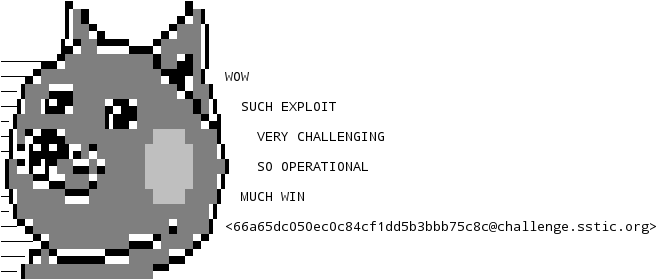
\includegraphics[width=14cm]{final.png}

La zone secrète du microcontrôleur contient donc l'adresse mail @challenge.sstic.org qu'il fallait trouver.

\section{Conclusion}

Le challenge SSTIC 2014 est avant tout centré sur les langages de type RISC. En effet, la trace USB initiale contient un programme ARM (le "R" signifiant initialement "RISC"). Ce programme interprète un autre programme RISC chiffré dans ses données, qui permet de déchiffrer une archive Zip. Cette archive contient un firmware pour un microcontrôleur accessible sur internet capable d'exécuter un troisième langage de type RISC, non documenté. C'est dans une zone protégée de la mémoire de ce microcontrôleur que se trouve l'adresse email qui permet de finir le challenge.

Ce document a décrit une solution qui utilise uniquement des logiciels libres : les programmes de GNU Coreutils\footnote{\url{http://www.gnu.org/software/coreutils/}}, objdump de GNU Binutils\footnote{\url{http://www.gnu.org/software/binutils/}}, et d'autres commandes comme file\footnote{\url{http://www.darwinsys.com/file/}}, xxd, etc. Les divers scripts qui ont été utilisés ont été écrit en Python\footnote{\url{https://www.python.org/}}. Les scripts les plus courts ont été directement recopiés dans les parties précédentes. Les plus longs se trouvent dans les annexes.

\section{Remerciements}

L'auteur souhaite tout d'abord remercier les concepteurs du challenge, qui fut très intéressant. Ce challenge a permis d'acquérir beaucoup de connaissances, par exemple dans les domaines suivants : assembleur ARM64, utilisation d'un firmware de microcontrôleur, etc.

Ensuite l'auteur souhaite remercier les personnes qui l'ont motivé à se lancer dans le challenge, par des phrases similaires à : "Ce qui est cool dans l'assembleur ARM64, ce sont les instructions amusantes comme LSL, UBFX et SBFIZ." et "De toutes façons, cette année, il faut une licence pro d'IDA pour pouvoir faire la partie ARM 64-bits.". Cette dernière affirmation est contredite par l'existence même de la solution présentée dans ce document. Celle-ci prouve en effet qu'il est possible d'utiliser objdump pour comprendre le code ARM64 (ainsi qu'un interpréteur ARM64 codé en Python qui offre des fonctionnalités similaires à la combinaison qemu-gdb).

L'auteur remercie enfin tous ceux qui l'ont aidé à l'écriture de ce document, que ce soit en indiquant les points à clarifier et les nombreuses fautes de français, ou en expliquant comment sont utilisés les "registres à décalage à rétroaction linaire" en cryptographie.

\clearpage

\begin{appendices}
\section{Introduction à l'assembleur ARM64}
\label{IntroARM64}

La syntaxe adoptée ici est celle de gas (GNU assembler), qui est la même que celle obtenue par le désassembleur d'objdump.

\subsection{Registres}

L'ARM64 est une architecture RISC dont chaque instruction fait 32 bits. Cette architecture dispose des registres suivants :
\begin{itemize}
\item 31 registres entiers de 64 bits (de \texttt{x0} à \texttt{x30}),
\item 32 registres du FPU de 128 bits (de \texttt{v0} à \texttt{v31}),
\item un "Program Counter" (\texttt{pc}),
\item un "Stack Pointer" (\texttt{sp}), qui est aligné sur 16 octets,
\item un "Zero Register" (\texttt{zr}), qui vaut toujours zéro,
\item 4 drapeaux, \texttt{NZCV} (Negative, Zero, Carry, oVerflow).
\end{itemize}

Par ailleurs, un mot ("word") fait 4 octets (32 bits), et donc le groupement de 2 octets s'appelle demi-mot ("halfword", 16 bits) et celui de 8 octets double-mot ("doubleword", 64 bits).

Les registres génériques sont des double-mots et sont nommés de \texttt{x0} à \texttt{x30}. Le mot de poids faible de chaque registre est nommé en remplaçant \texttt{x} par \texttt{w} et donc de \texttt{w0} à \texttt{w30}.

La convention d'appel des procédures indique que les registres génériques ont les rôles suivants.
\begin{itemize}
\item \texttt{x0} à \texttt{x7}, paramètres et valeurs de retour.
\item \texttt{x8}, "Indirect result location register". Sur Linux ce registre contient le numéro d'appel système à effectuer lors de l'utilisation de l'instruction "\texttt{svc \#0x0}".
\item \texttt{x9} à \texttt{x15}, registres "temporaires" qui peuvent être écrasés lors d'un appel de procédure.
\item \texttt{x16} et \texttt{x17}, "Intra-procedure-call scratch register" (\texttt{IP0} et \texttt{IP1}).
\item \texttt{x18}, "platform, ABI-specific register".
\item \texttt{x19} à \texttt{x28}, les registres garantis inchangés lors d'un appel de fonction. Toute fonction devrait sauvegarder et restaurer la valeur de chacun de ces registres qu'elle utilise.
\item \texttt{x29}, "Frame Pointer", \texttt{fp}, est un point de repère sur la pile qui permet d'avoir simplement la notion de "stack frame", de "variables locales sur la pile", etc. En particulier cela permet de créer des "stack traces" lors du débogage de programmes.
\item \texttt{x30}, "Link Register", \texttt{lr}, contient l'adresse de retour.
\end{itemize}
En pratique, une application exécutée en mode utilisateur sur un système Linux utilise principalement \texttt{x0} à \texttt{x8} et \texttt{x19} à \texttt{x30}.

Le document "Procedure Call Standard for the ARM 64-bit Architecture"\footnote{\url{http://infocenter.arm.com/help/topic/com.arm.doc.ihi0055b/IHI0055B_aapcs64.pdf}} définit avec plus de détails tout cela.

\subsection{Instructions spécifiques de l'ARM64}

Voici quelques subtilités de l'assembleur ARM64, au niveau des instructions :
\begin{itemize}
\item Le "Logical Shift Left" (LSL) est quasi-omniprésent car peut être intégré de base à beaucoup d'instructions. Par exemple \texttt{add x5, x19, x5, lsl \#3} correspond en C à \texttt{x5 = x19 + (x5 \lsl 3)}.
\item L'accès à la mémoire en mode "registre + offset" fonctionne à peu comme pour l'assembleur x86. Par exemple \texttt{[sp,\#16]} correspond à l'adresse \texttt{sp + 16} et \texttt{[x0,x1,lsl \#3]} à \texttt{x0 + (x1 \lsl 3)}.
\item La notation "pre-indexed" \texttt{[base,\#imm]!} permet de mettre à jour la valeur d'un registre avant que celui-ci ne soit utilisé. Ainsi \texttt{stp x29, x30, [sp,\#-16]!} décrémente \texttt{sp} de 16 puis écrit \texttt{x29} et \texttt{x30} à l'adresse obtenue.
\item La notation "post-indexed" \texttt{[base],\#imm} permet de mettre à jour la valeur d'un registre après que celui-ci soit utilisé. Ainsi \texttt{ldp x29, x30, [sp],\#16} charge \texttt{x29} et \texttt{x30} depuis l'adresse \texttt{sp} et incrémente \texttt{sp} de 16.
\item Les instructions \texttt{add} et \texttt{sub} n'agissent pas sur les drapeaux (\texttt{NZCV}) mais celles suffixées par \texttt{s} (\texttt{adds} et \texttt{subs}) si, tout comme \texttt{cmn} ("CoMpare with Negative) et \texttt{cmp} ("CoMPare").
\item \texttt{cmp a, b} calcule la différence entre \texttt{a} et \texttt{b} en effectuant \texttt{a + not(b) + 1}. Cela a pour conséquence directe que le "Carry Flag" est mis à un si \texttt{a >= b} et à zéro si \texttt{a < b}. C'est le contraire de la convention employée pour x86.
\item \texttt{sxtw} permet d'étendre un mot en un double-mot en conservant le signe (ie. le bit de poids fort est répliqué sur tous les bits du mot de poids fort). Il s'agit d'une instruction (\texttt{sxtw x0, w0}) aussi bien que d'une notation (\texttt{add x7, x0, w2, sxtw}).
\item \texttt{uxtw} permet d'étendre un mot en un double-mot de manière non-signée (d'où le \texttt{u}, pour "unsigned"). \texttt{uxtb} fait la même chose pour un octet.
\end{itemize}

La liste des instructions est donnée par le document "ARMv8 Instruction Set Overview" \footnote{\url{http://board.flatassembler.net/download.php?id=5698}}

Tout ceci permet de comprendre la "structure conventionnelle" d'une procédure ARM64 :
\begin{verbatim}
stp x29, x30, [sp,#-64]!    ; Sauvegarde de fp et lr sur la pile
mov x29, sp                 ; "fp = sp", définition du nouveau cadre de pile
stp x19, x20, [sp,#16]      ; Sauvegarde des registres x19 à x24 (s'ils sont utilisés)
stp x21, x22, [sp,#32]
stp x23, x24, [sp,#48]
...                         ; Code de la fonction
mov x0, #0x2a               ; Définition de la valeur de retour
ldp x19, x20, [sp,#16]      ; Restauration des registres x19 à x24 sauvegardés
ldp x21, x22, [sp,#32]
ldp x23, x24, [sp,#48]
ldp x29, x30, [sp],#64      ; Restauration de fp, lr et sp
ret                         ; ou "bx lr", qui effectue un branchement en lr
\end{verbatim}

L'appel d'une procédure, effectuée par \texttt{bl adresse}, effectue les opérations \texttt{lr = pc} et \texttt{pc = adresse}.

\subsection{Interface avec Linux}

Dans le cadre du challenge, l'application analysée s'exécute dans un environnement Linux. Dans ce cadre, il n'existe que deux interfaces avec le système d'exploitation : l'environnement initial du programme (valeur des registres et contenu de la pile) et l'utilisation d'appels systèmes (communément appelés "syscall").\footnote{En réalité avec le vDSO il existe une troisième manière d'interagir avec le noyau, mais ceci dépasse le cadre de ce document.}

L'environnement initial est la manière qu'à Linux de passer les paramètres de la ligne de commande à l'application. Avec la convention usuelle de définition de la fonction \texttt{main} en C, à savoir :
\begin{verbatim}
int main(int argc, char **argv, char **envp);
\end{verbatim}
la pile contient au lancement du programme \texttt{argc}, puis \texttt{argv[0]} à \texttt{argv[argc - 1]}, puis \texttt{NULL}, \texttt{envp[0]} ... \texttt{NULL}.
Dans glibc 2.19, ceci est documenté et implémenté dans \texttt{ports/sysdeps/aarch64/start.S}\footnote{\url{https://sourceware.org/git/?p=glibc.git;a=blob;f=ports/sysdeps/aarch64/start.S;hb=9a869d822025be8e43b78234997b10bf0cf9d859}}.

Pour effectuer un appel système, le programme utilise l'instruction "\texttt{svc \#0x0}" avec le numéro du syscall dans \texttt{x8} et les paramètres dans les registres  \texttt{x0} à \texttt{x6}. La valeur de retour du syscall est dans \texttt{x0}. Dans glibc 2.19, la fonction C \texttt{syscall(int nr, ...)} est implémentée dans \texttt{ports/sysdeps/unix/sysv/linux/aarch64/syscall.S}\footnote{\url{https://sourceware.org/git/?p=glibc.git;a=blob;f=ports/sysdeps/unix/sysv/linux/aarch64/syscall.S;hb=9a869d822025be8e43b78234997b10bf0cf9d859}}.
Les sources de Linux contiennent la liste des syscalls utilisés par ARM64 dans le fichier \\
\texttt{include/uapi/asm-generic/unistd.h}\footnote{\url{https://git.kernel.org/cgit/linux/kernel/git/torvalds/linux.git/tree/include/uapi/asm-generic/unistd.h?id=455c6fdbd219161bd09b1165f11699d6d73de11c}}\footnote{Si cette liste était spécifique à ARM64, elle serait dans \texttt{arch/arm64/include/uapi/asm/unistd.h}, mais comme elle est partagée par plusieurs architectures, elle se trouve directement dans \texttt{include/uapi/asm-generic}.}.

\section{Code Python de l'interpréteur ARM64}

L'interpréteur ARM64 que l'auteur a créé au cours du challenge utilise trois modules Python.
\begin{itemize}
\item \texttt{arm64emu.py} permet d'exécuter des instructions ARM64 en traçant éventuellement l'exécution suivant différents niveaux de granularité (par exemple il est possible de n'afficher que les syscalls, ou le graphe des appels, ou les instructions, ou les branchements, ou n'importe quelle combinaison de tout ceci).
\item \texttt{load\_objdump.py} permet de lire un fichier issu d'un désassemblage par objdump et d'en extraire une liste d'instructions.
\item \texttt{memory\_map.py} permet de gérer la mémoire virtuelle d'un programme.
\end{itemize}

\subsection{Contenu de \texttt{load\_objdump.py}}

\pyinput{2_arm64/load_objdump.py.inc.tex}

\subsection{Contenu de \texttt{memory\_map.py}}

\pyinput{2_arm64/memory_map.py.inc.tex}

\subsection{Contenu de \texttt{arm64emu.py}}

\pyinput{2_arm64/arm64emu.py.inc.tex}

\section{Décodeur du langage de type RISC de \texttt{badbios.bin}}

La section \ref{arm64risc} donne trois tables (\ref{badbiosRISCtable}, \ref{badbiosRISCcondbranch} et \ref{badbiosRISCsyscall}) qui permettent de décoder les instructions interprétées par \texttt{badbios.bin} pour exécuter l'algorithme de déchiffrement. Un extrait du décodage obtenu avec des commentaires et des étiquettes est disponible au début de la section \ref{badbiosRISCDecrypt}. Voici un script Python qui implémente ce décodage.

\pyinput{2_arm64/disasm_badbiosrisc.py.inc.tex}

\section{Décodage complet du firmware}

Voici un décodage complet des instructions du firmware \texttt{mcu/fw.hex} (cf. \ref{firmzip}). Chaque fonction est associée à un bloc de pseudo-code explicatif à sa droite.

\verbatiminput{3_mcu/firmware.txt}

\end{appendices}

\end{document}
